\documentclass[11pt,a4paper]{article}
\textheight245mm
\textwidth170mm
\hoffset-21mm
\voffset-15mm
\parindent0pt
\usepackage[utf8]{inputenc}
\usepackage{dsfont}
\usepackage{graphicx}
\usepackage{caption}
\usepackage{subcaption}
\usepackage{fancyhdr}
\usepackage{amsmath,amsfonts,amssymb}
\usepackage{float}
\usepackage{dsfont}
\usepackage{cancel}
\usepackage[french]{babel}
\usepackage[maxalphanames=99, maxnames=99, backend=bibtex, style=alphabetic, sorting=ynt]{biblatex}
\addbibresource{rapport.bib}
\usepackage[hidelinks]{hyperref} 
\hypersetup{
  colorlinks   = true,    % Colours links instead of ugly boxes
  urlcolor     = blue,    % Colour for external hyperlinks
  linkcolor    = black,    % Colour of internal links
  citecolor    = black      % Colour of citations
}
\usepackage{/home/hazdard/Documents/Tex/zephyr}
\pagestyle{fancy}

\usepackage{array,multirow,makecell}
\setcellgapes{4pt}
\makegapedcells
\newcolumntype{R}[1]{>{\raggedleft\arraybackslash }b{#1}}
\newcolumntype{L}[1]{>{\raggedright\arraybackslash }b{#1}}
\newcolumntype{C}[1]{>{\centering\arraybackslash }b{#1}}

\renewcommand{\headrulewidth}{1pt}
\fancyhead[C]{}
\fancyhead[L]{L3 - 2023/2024}
\fancyhead[R]{D.E.R Mathématiques}

\renewcommand{\footrulewidth}{1pt}
\fancyfoot[C]{\thepage} 
\fancyfoot[L]{T. Abrial, S. Ben-Arous, M. Bordet}
\fancyfoot[R]{E.N.S Paris-Saclay}

\title{\textbf{Étude expérimentale et théorique de modèles de percolation}}
\date{22 Avril 2024}
\author{Théo Abrial, Sacha Ben-Arous, Mathis Bordet}

\begin{document}

\maketitle 
\tableofcontents
\newpage
\section{Présentation du modèle}

La théorie de la percolation est un domaine de physique mathématique qui vise à étudier la géométrie et la connectivité de structures et matériaux, en se demandant par exemple si un liquide peut traverser une pierre ponce, ou si un charbon laisse passer des gaz dans le cas d'un masque à gaz. \\
Dans un souci de simplicité, on ne s'intéresse pas au comportement de chaque atome du matériau, mais plutôt à sa structure globale, et on modélise souvent ces structures par des labyrinthes aléatoires. 
Plus précisemment, on considérera un graphe aléatoire où deux sommets ont une certaine probabilité d'être reliés. En théorie ce graphe est infini, mais ce ne sera pas le cas dans la partie expérimentale. Dans le rapport suivant, on s'attachera à étudier certaines propriétés de ces graphes aléatoires, en particulier la probabilité d'existence d'une composante connexe infinie, auquel cas on parlera de ``percolation". On se placera toujours sur le graphe $\mathbb{Z}^d$, ou bien sur une section finie de ce dernier. 

\section{Modélisation informatique}
\ \ \ \ \ On va étudier le problème de percolation en dimension $2$ grâce à la modélisation suivante : on se donne une grille de longueur $l$, de hauteur $h$, et chaque case de la grille a une probabilité $p$ d'être ouverte, indépendamment des autres cases, dans ce cas sa valeur sera mise à \verb|True|, sinon à \verb|False|. On se demande alors si il y a percolation, c'est à dire si il est possible de relier le haut et le bas de la grille, en passant uniquement par des cases ouvertes, en se déplaçant sur l'axe vertical et horizontal, mais pas en diagonale. Dans un premier temps, on mettra en évidence l'existence d'une probabilité critique, puis on observera ensuite différentes propriétés du modèle. \\
Pour faire une simulation, on tire une grille au hasard suivant les paramètres $l,h$ et $p$, puis on fait un parcours en profondeur de la grille à l'aide d'une pile pour déterminer les chemins explorés depuis la hauteur initiale, à la manière d'un fluide qui se propage. Le code utilisé est disponible \href{https://github.com/Hazdard/Percolation/blob/main/percolation.ipynb}{ici}.

\subsection{Probabilité critique et diagramme de phase}

Tout d'abord, les simulations numériques permettent de mettre en évidence un phénomène bien connu en percolation : l'existence d'un seuil critique, défini par $p_c = \sup{ \{p, \ \mathbb{P}_p[\text{percolation]}=0 \} }$, où $ \mathbb{P}_p$ est la mesure de probabilité correspondant au tirage de la grille. $p_c$ représente le seuil à partir duquel la probabilité de percolation est non nulle. Attention cependant, le comportement au niveau de $p_c$ est inconnu en général, et il est conjecturé que sur $\mathbb{Z}^d$, il n'y a presque sûrement pas percolation à $p=p_c$. Pour observer ce seuil, on génère une grille sur laquelle on augmente progressivement la valeur de $p$, où l'on a représenté en bleu les chemins que l'on peut parcourir depuis le haut de la grille : 

\begin{figure}[htbp]
    \centering
    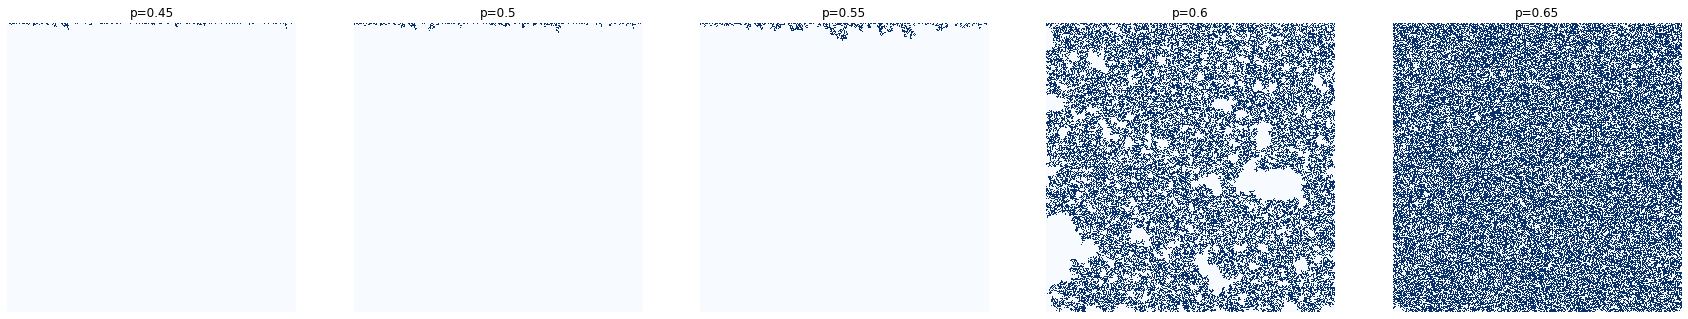
\includegraphics[width=1 \textwidth]{./Pictures/evolution.png}
    \caption{Évolution de la percolation sur une grille $500\times 500$ en fonction de la probabilité d'ouverture}
    \label{fig:evol}
\end{figure}

Ces simulations mettent en évidence que la probabilité critique pour notre modélisation est autour de $0.6$\ . Attention cependant, dans la partie théorique qui suit, on montrera que la probabilité critique vaut $0.5$, mais le modèle qui y sera étudié est légeremment différent car ce sont les arêtes qui y seront ouvertes ou fermées, et non pas les cases. Ici, dans ce modèle dit de ``percolation par sites'', la valeur critique exacte n'est pas explicitement connue. \\

On peut ensuite calculer expérimentalement le diagramme de phase de notre modèle, c'est à dire la probabilité de percolation en fonction de la probabilité d'ouverture; et le comparer au diagramme de phase théorique de la percolation ``classique'' précédemment évoquée. On constate que dans le modèle par sites, la percolation presque sûre est atteinte bien plus rapidement. Une étude théorique approfondie de ce diagramme de phase est réalisée en section $3$.


\begin{figure}[H]
    \centering
    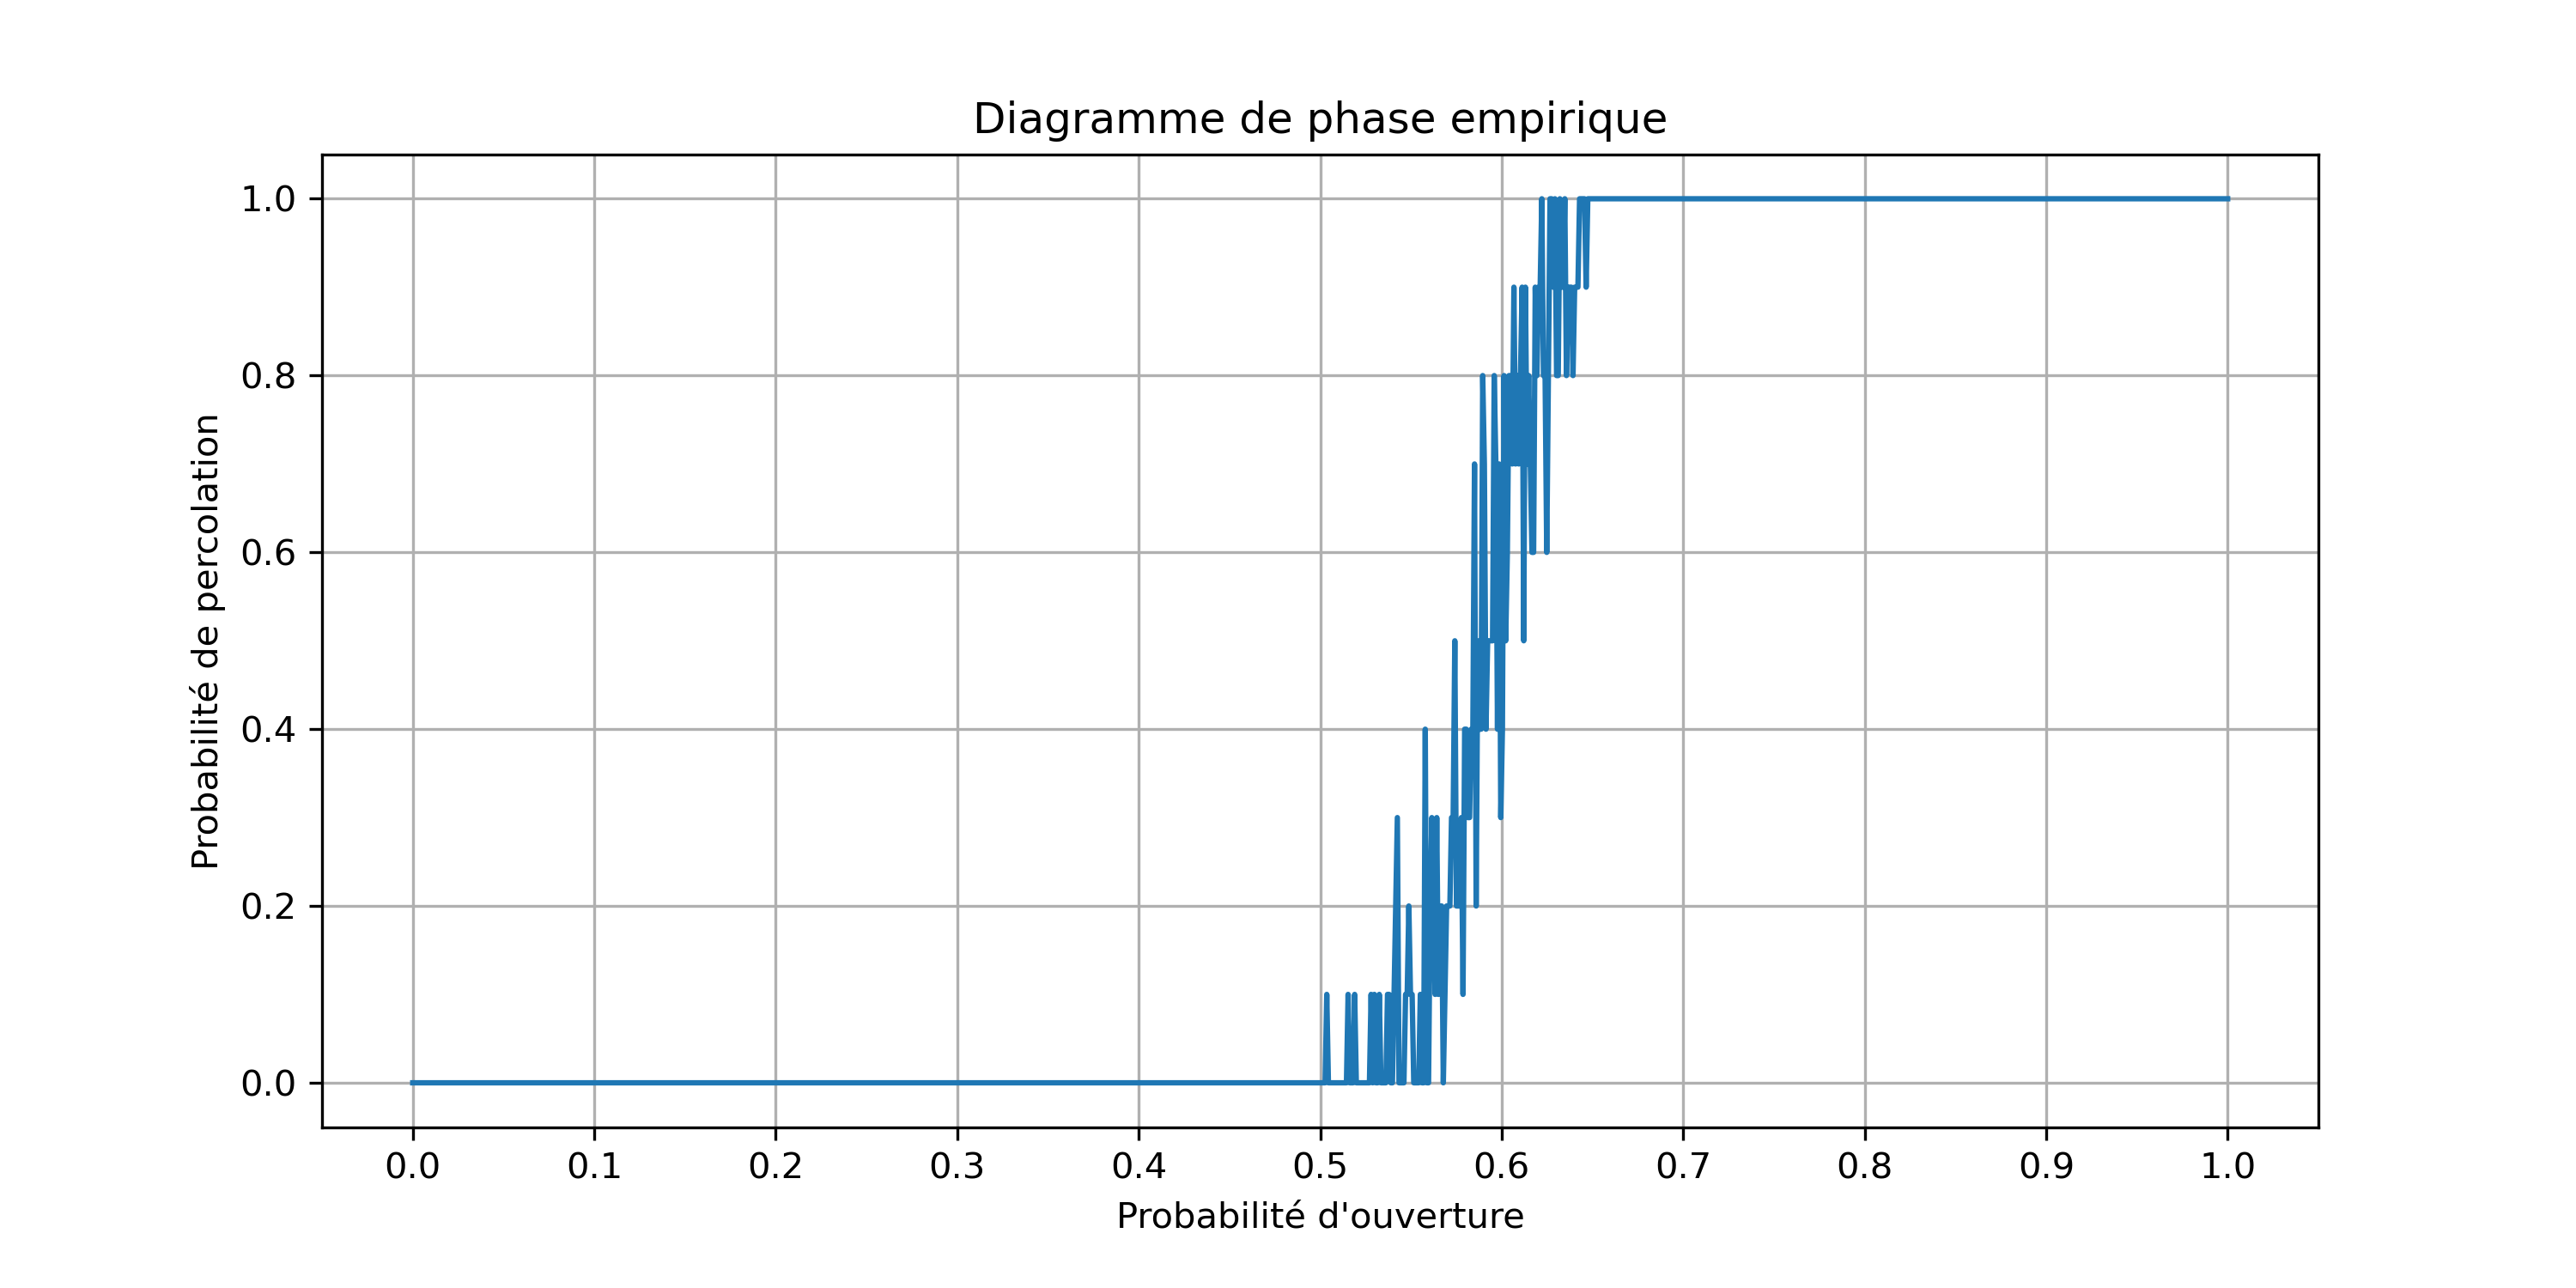
\includegraphics[width=0.5 \textwidth]{./Pictures/percolation_probability.png}
    \caption{Diagramme de phase expérimental pour une grille $100\times 100$}
    \label{fig:phase}
\end{figure}


\begin{figure}[H]
    \centering
    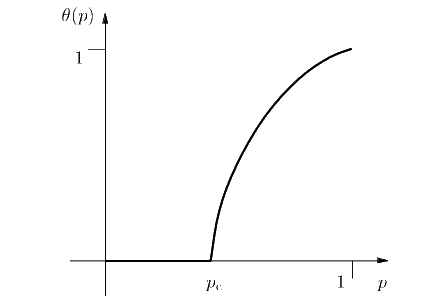
\includegraphics[width=0.4 \textwidth]{./Pictures/ph_th.png}
    \caption{Diagramme de phase théorique dans le cas de percolation standard \cite{grimmett}}
    \label{fig:phase_th}
\end{figure}

\subsection{Plus grande composante connexe}
\ \ \ \ \ Dans la partie théorique suivante, nous aurons besoin d'un résultat d'unicité de la plus grande composante connexe lorsqu'il y a percolation, c'est à dire unicité de la composante connexe infinie car en théorie la grille est infinie. 
\begin{figure}[H]
\centering
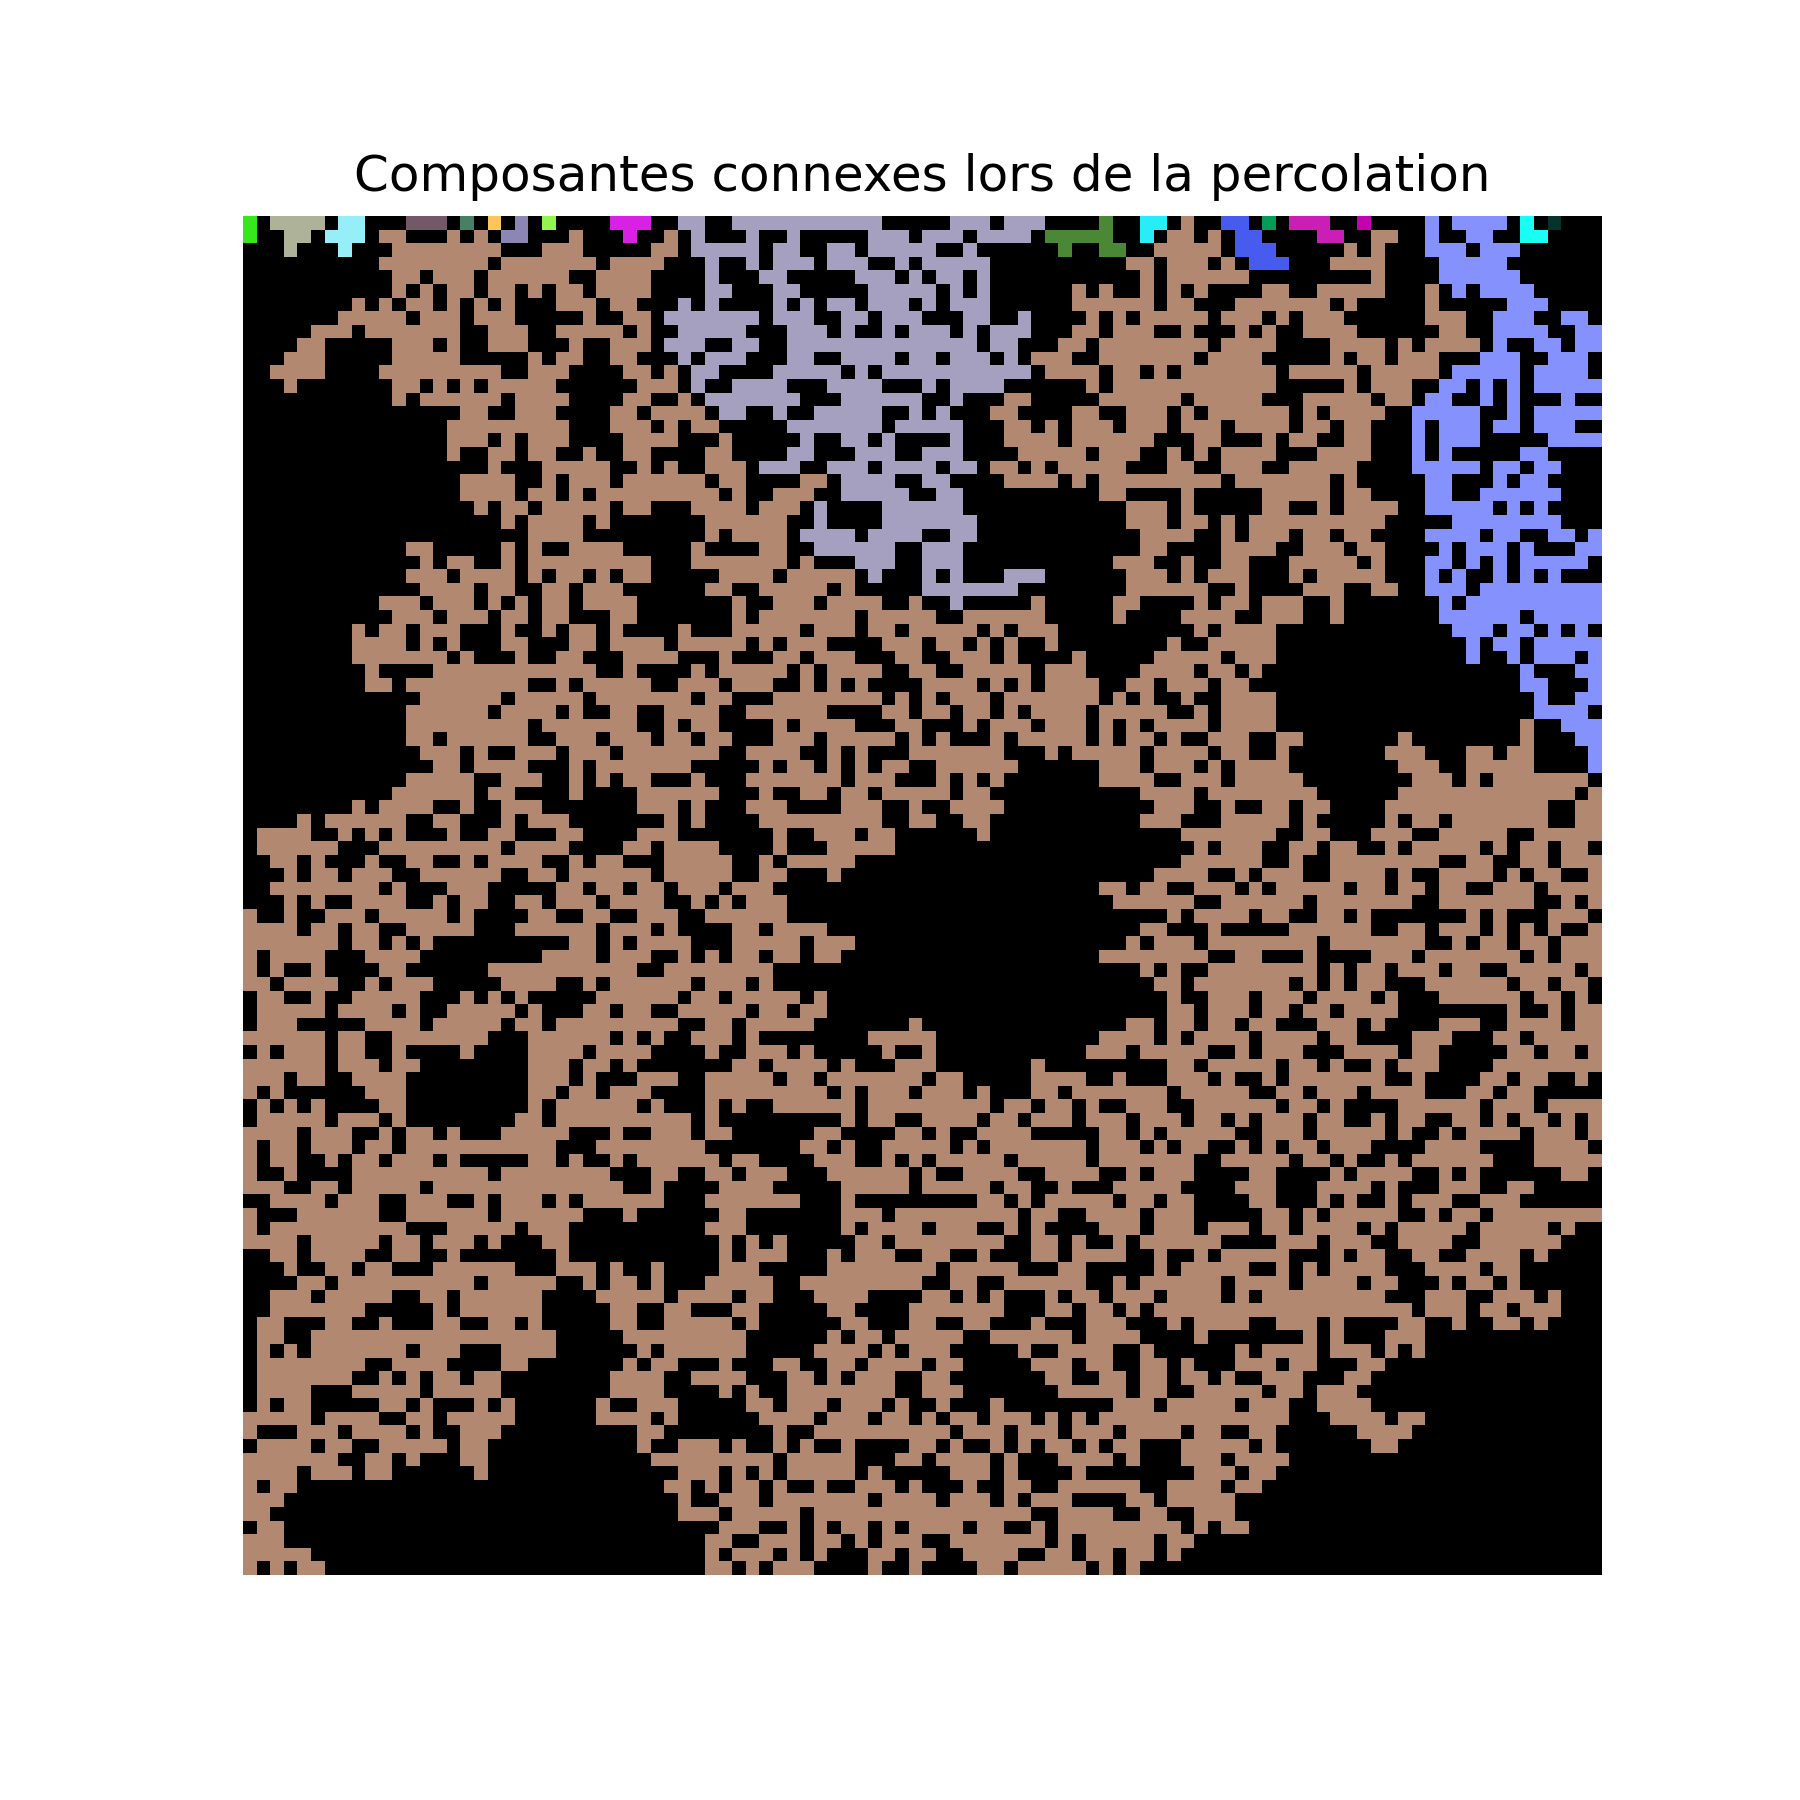
\includegraphics[width=.3333\textwidth]{./Pictures/cc100.png}\hfill
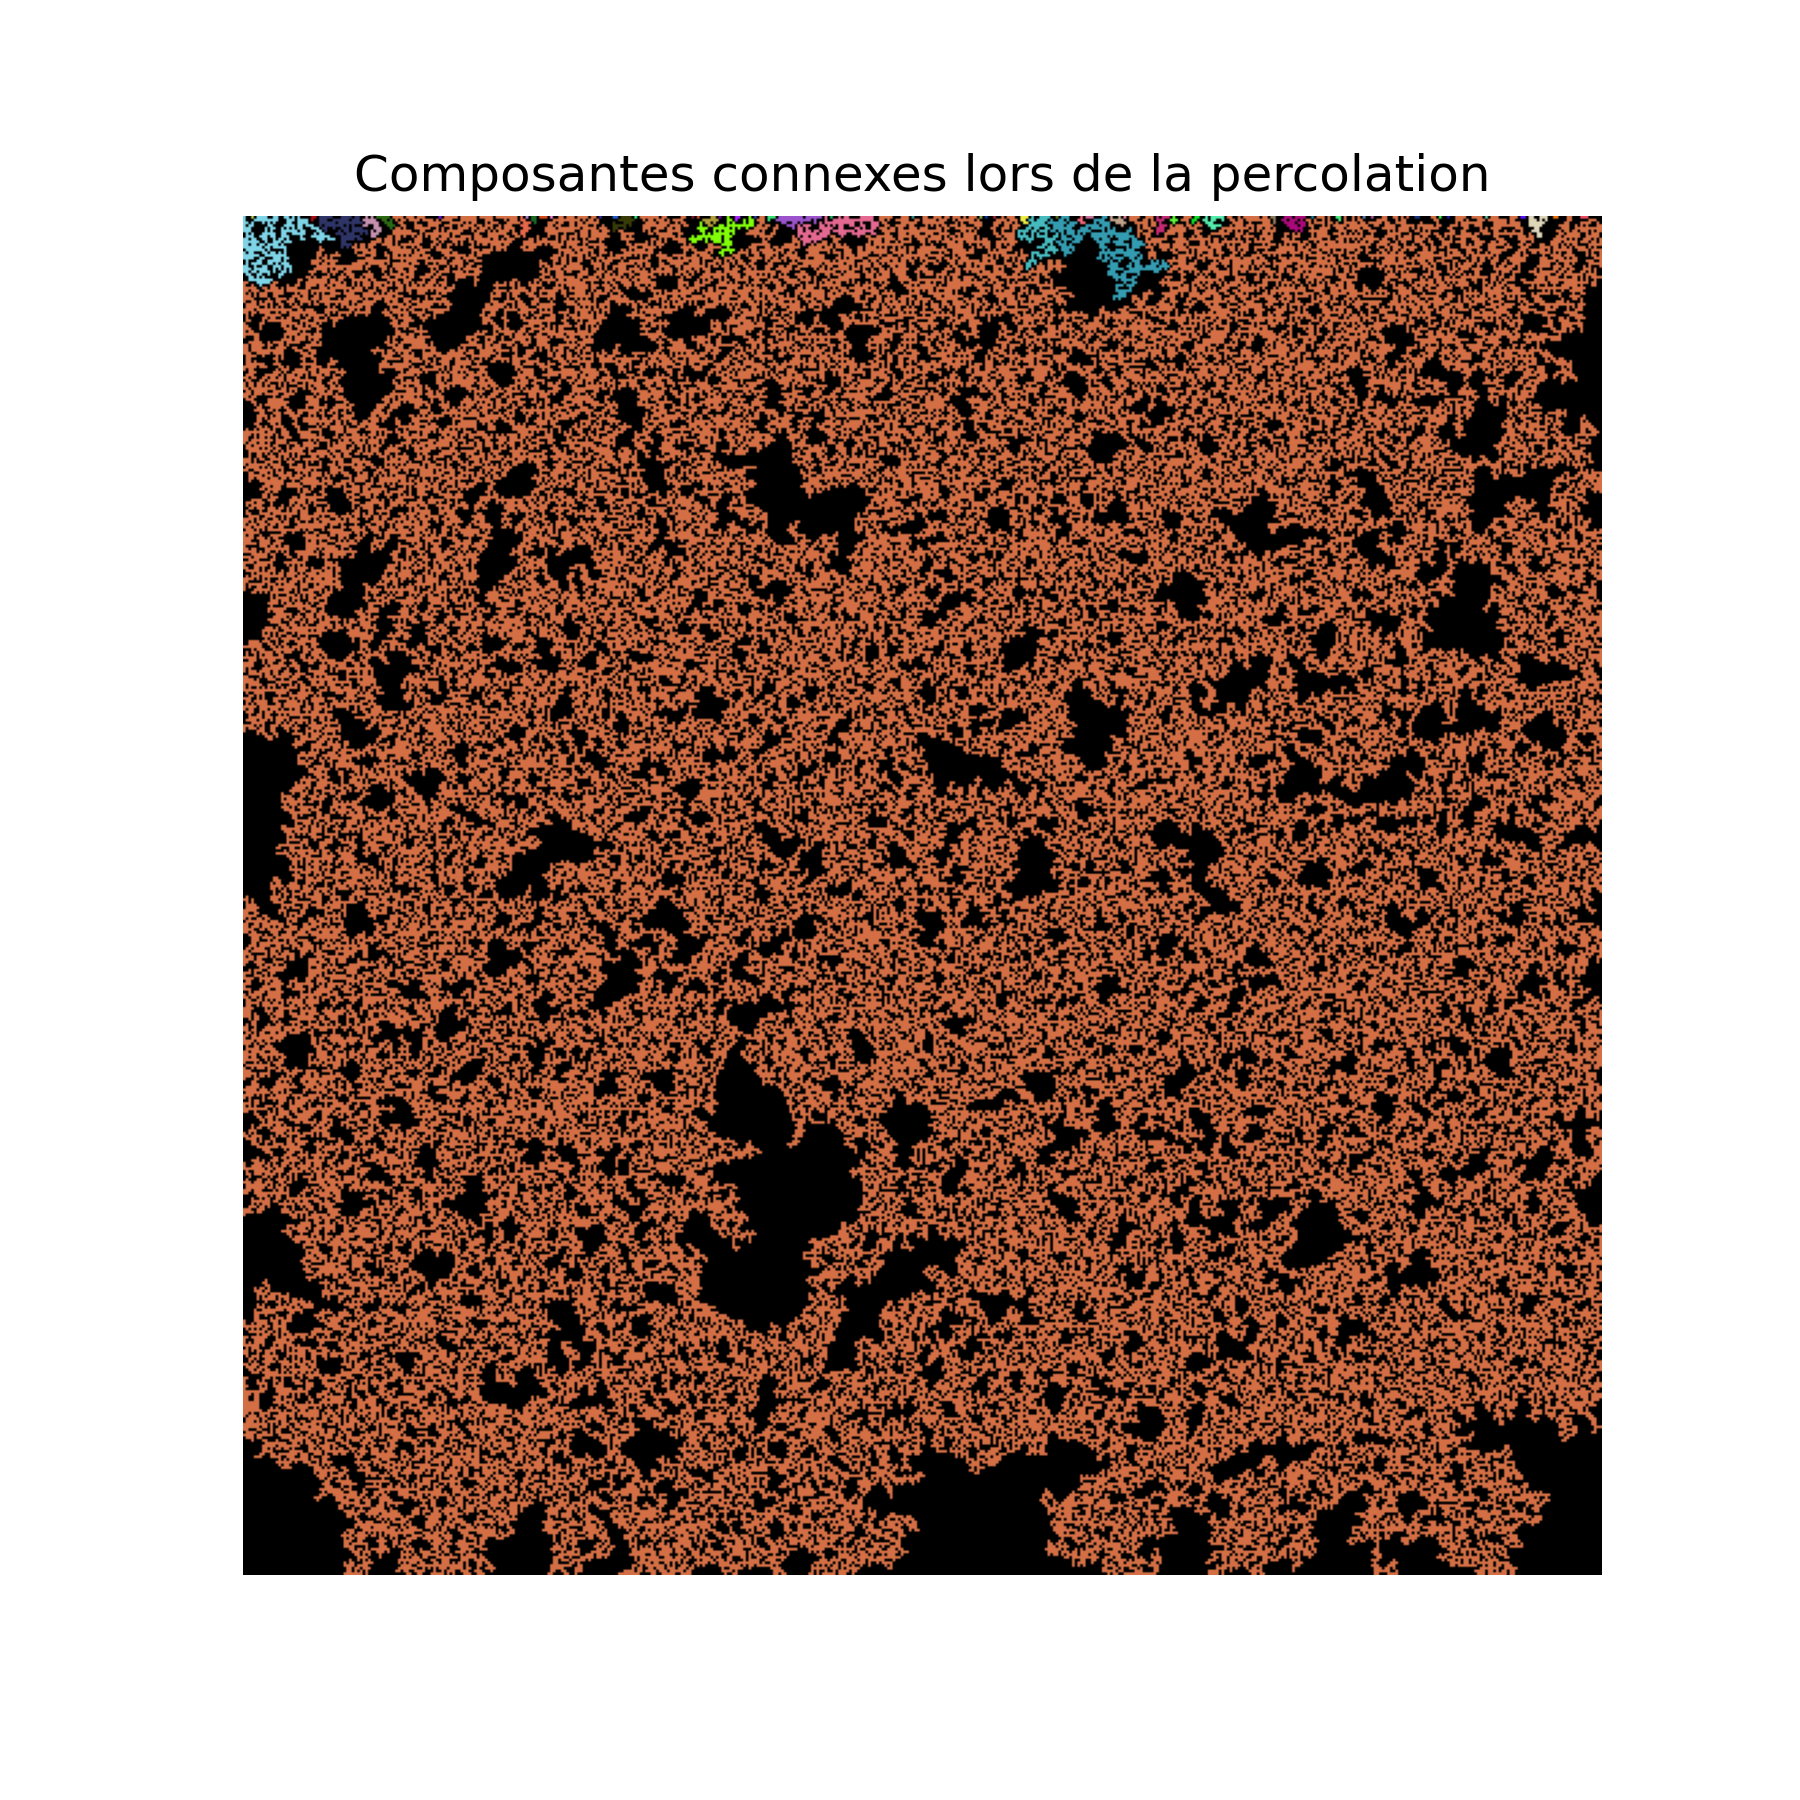
\includegraphics[width=.3333\textwidth]{./Pictures/cc500.png}\hfill
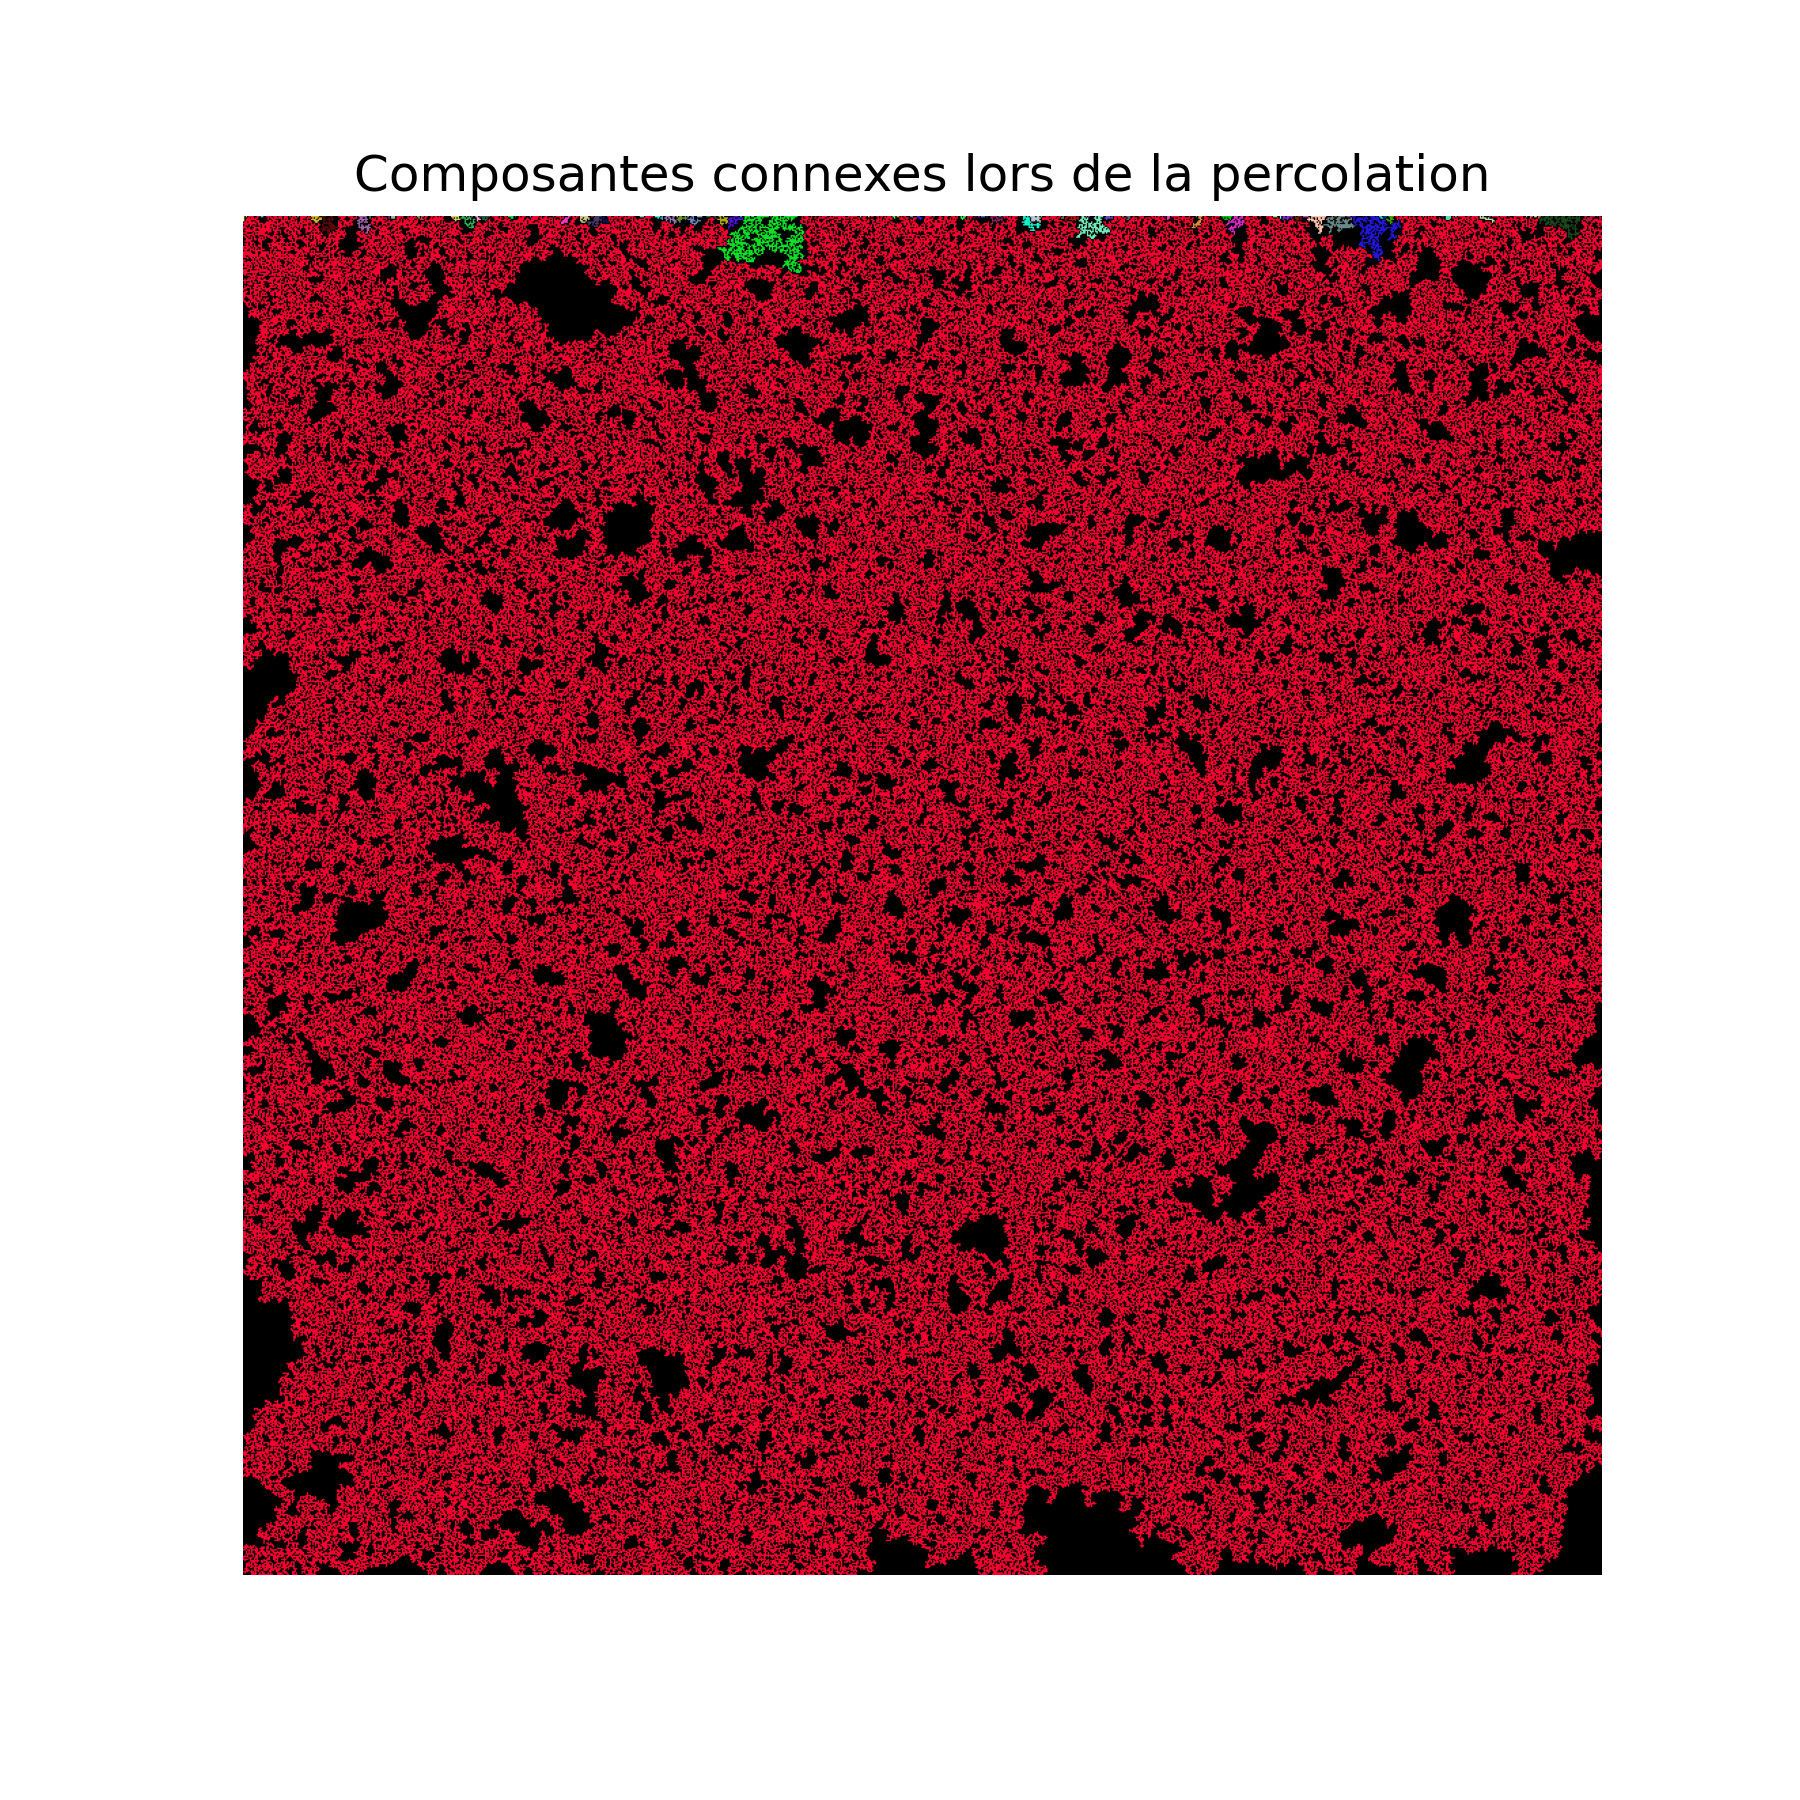
\includegraphics[width=.3333\textwidth]{./Pictures/cc1000.png}
\caption{Composantes connexes coloriées sur des grilles carrées de taille $100$, $500$ et $1000$ à $p=0.6$}
\label{fig:cc}

\end{figure}


Au vu de la difficulté de la preuve rigoureuse de ce lemme, on se propose plutôt de le mettre en évidence expérimentalement : les graphes ci-dessus ont leurs composantes connexes coloriés, on observe bien qu'il y a unicité de la composante qui atteint le bas de la grille. \\
 
On complète ces observations par le graphe de la profondeur maximale atteinte, ainsi que celui de la taille maximale/moyenne des composantes connexes, la taille d'une composante étant le nombre de cases qu'elle contient. Le premier corrobore les observations sur la probabilité critique $p_c \simeq 0.6$ à partir de laquelle la profondeur maximale atteinte est celle de la grille. Dans le second graphe, on observe en particulier qu'au voisinage de $p_c$, la taille maximale est nettement supérieure à celle moyenne, ce qui met encore en évidence que la composante maximale qui percole est exceptionnelle dans la grille. Puis pour $p$ proche de $1$, les deux valeurs convergent vers la taille du graphe, car la connectivité est alors suffisamment grande pour que presque toutes les cases soient reliées, conduisant ainsi à une unique composante connexe qui recouvre la quasi-totalité de la grille.


\begin{figure}[H]

\centering
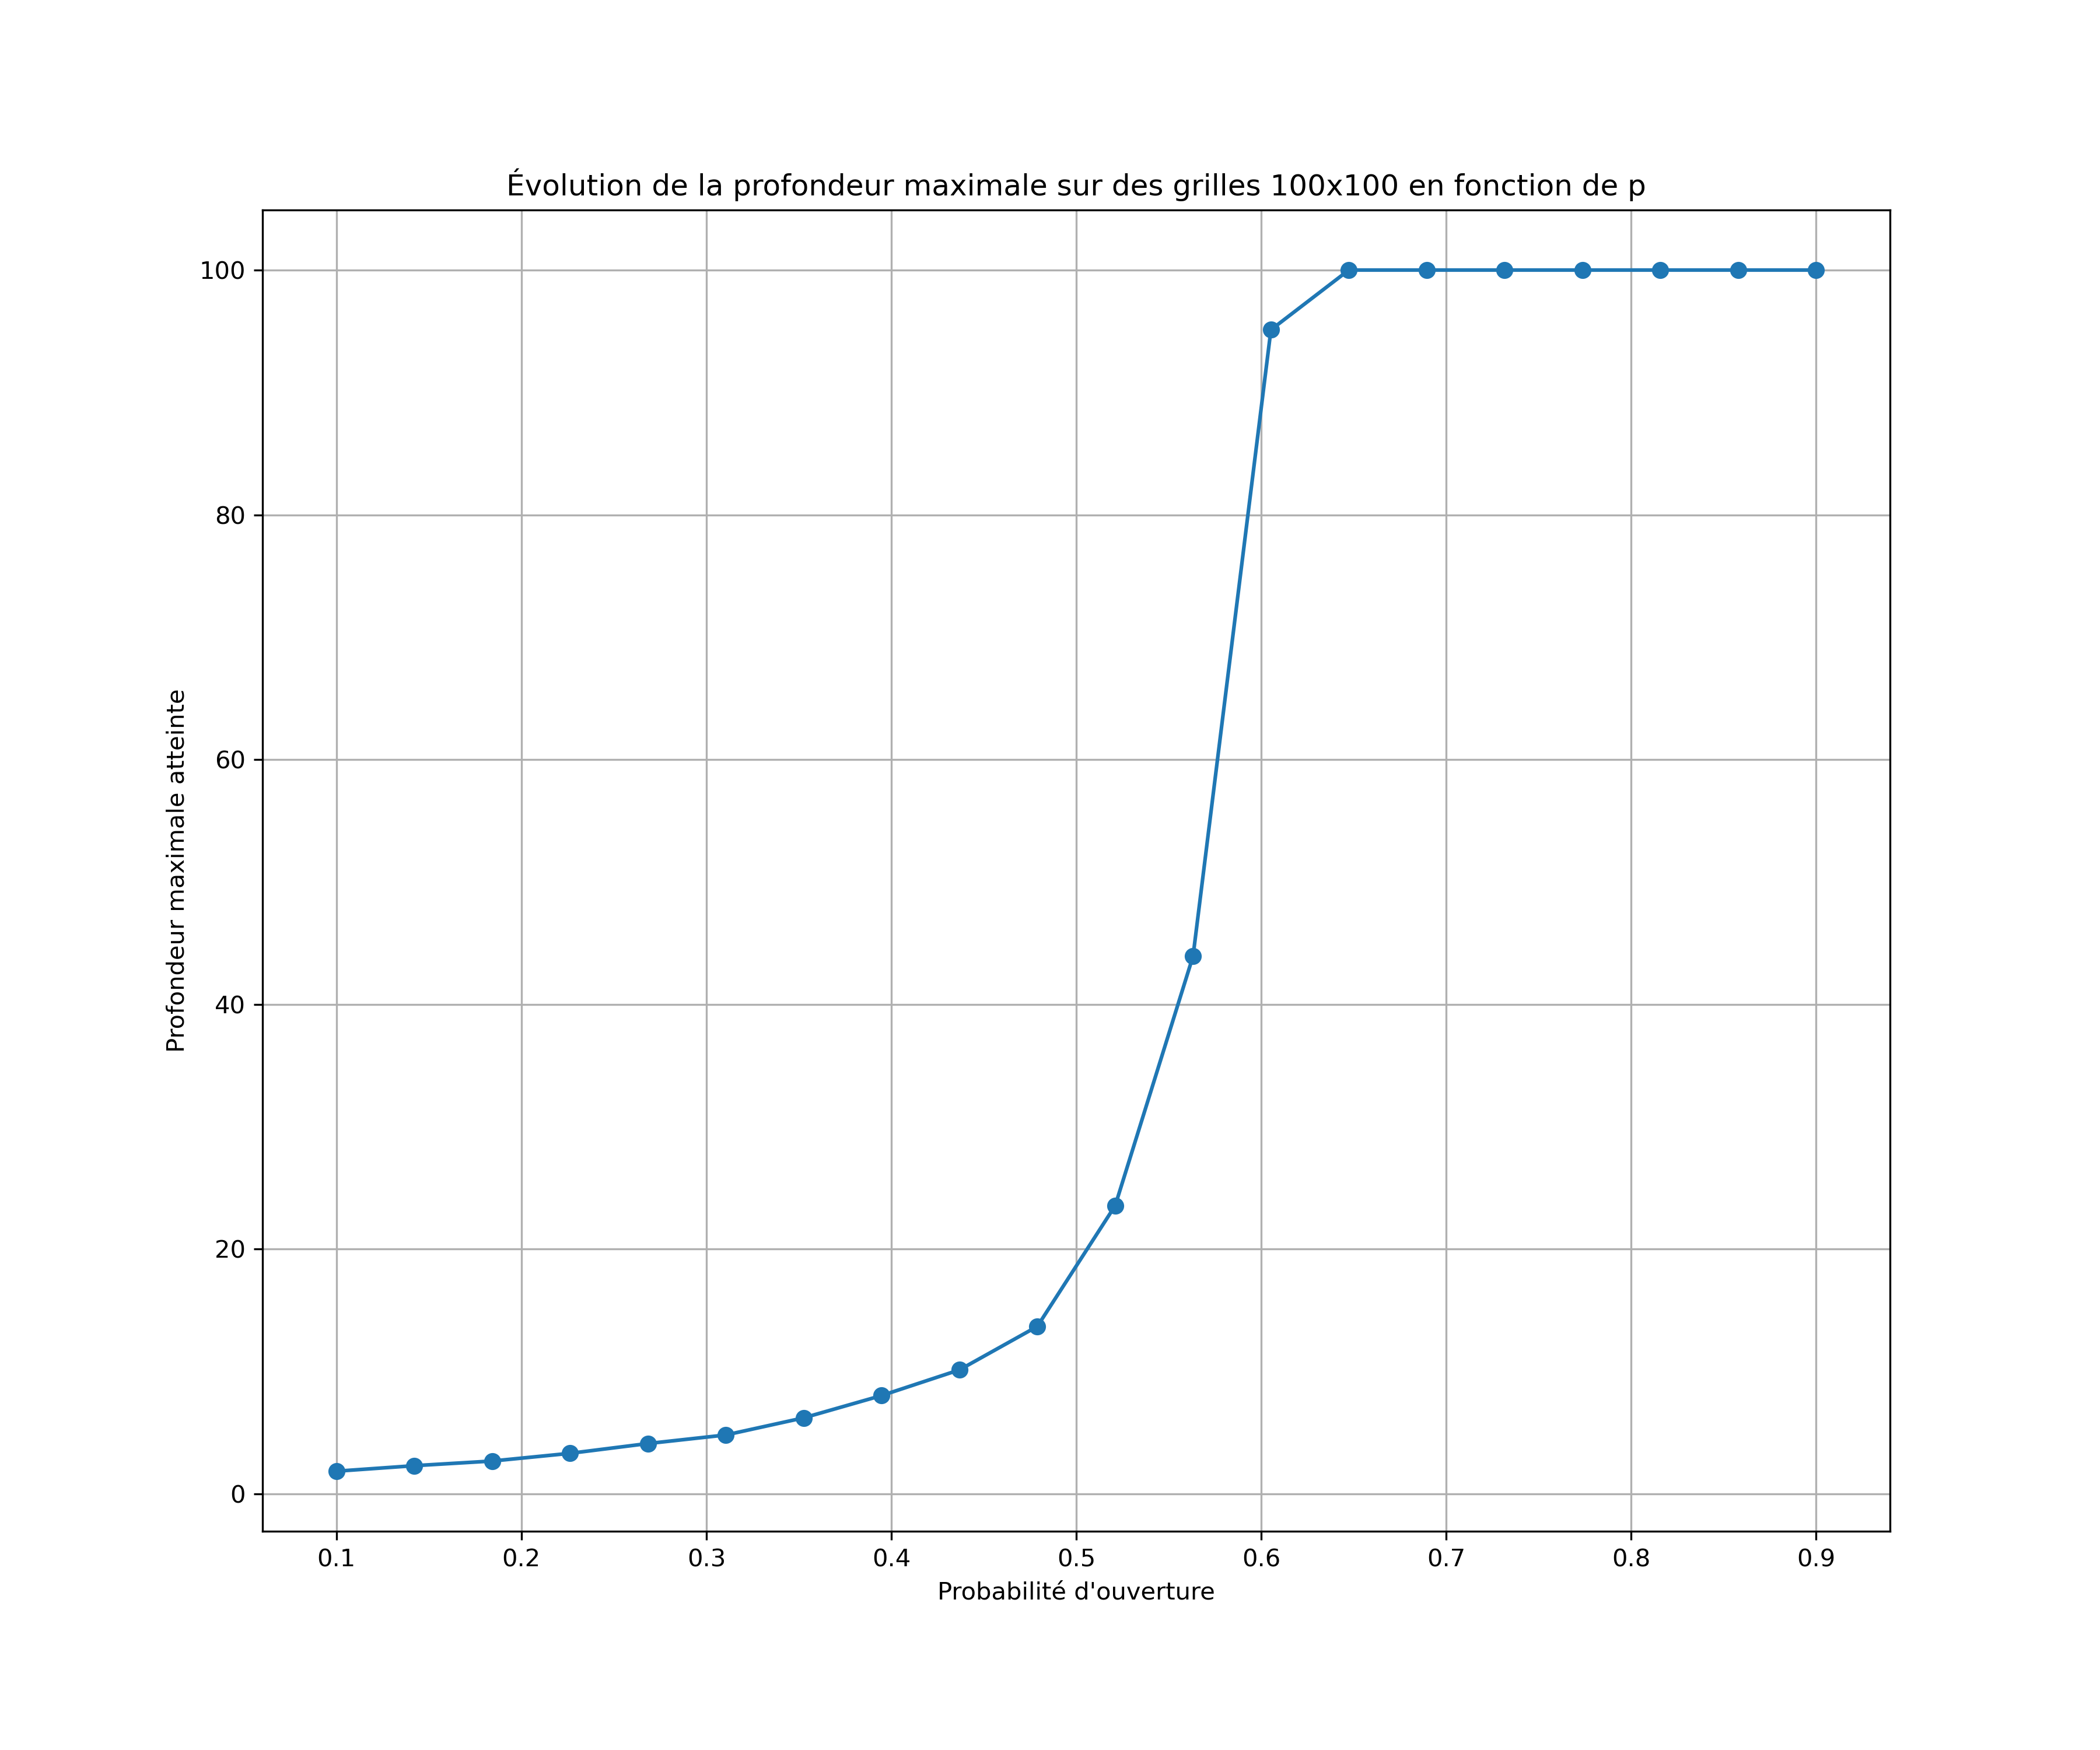
\includegraphics[width=.5\textwidth]{./Pictures/profondeur.png}\hfill
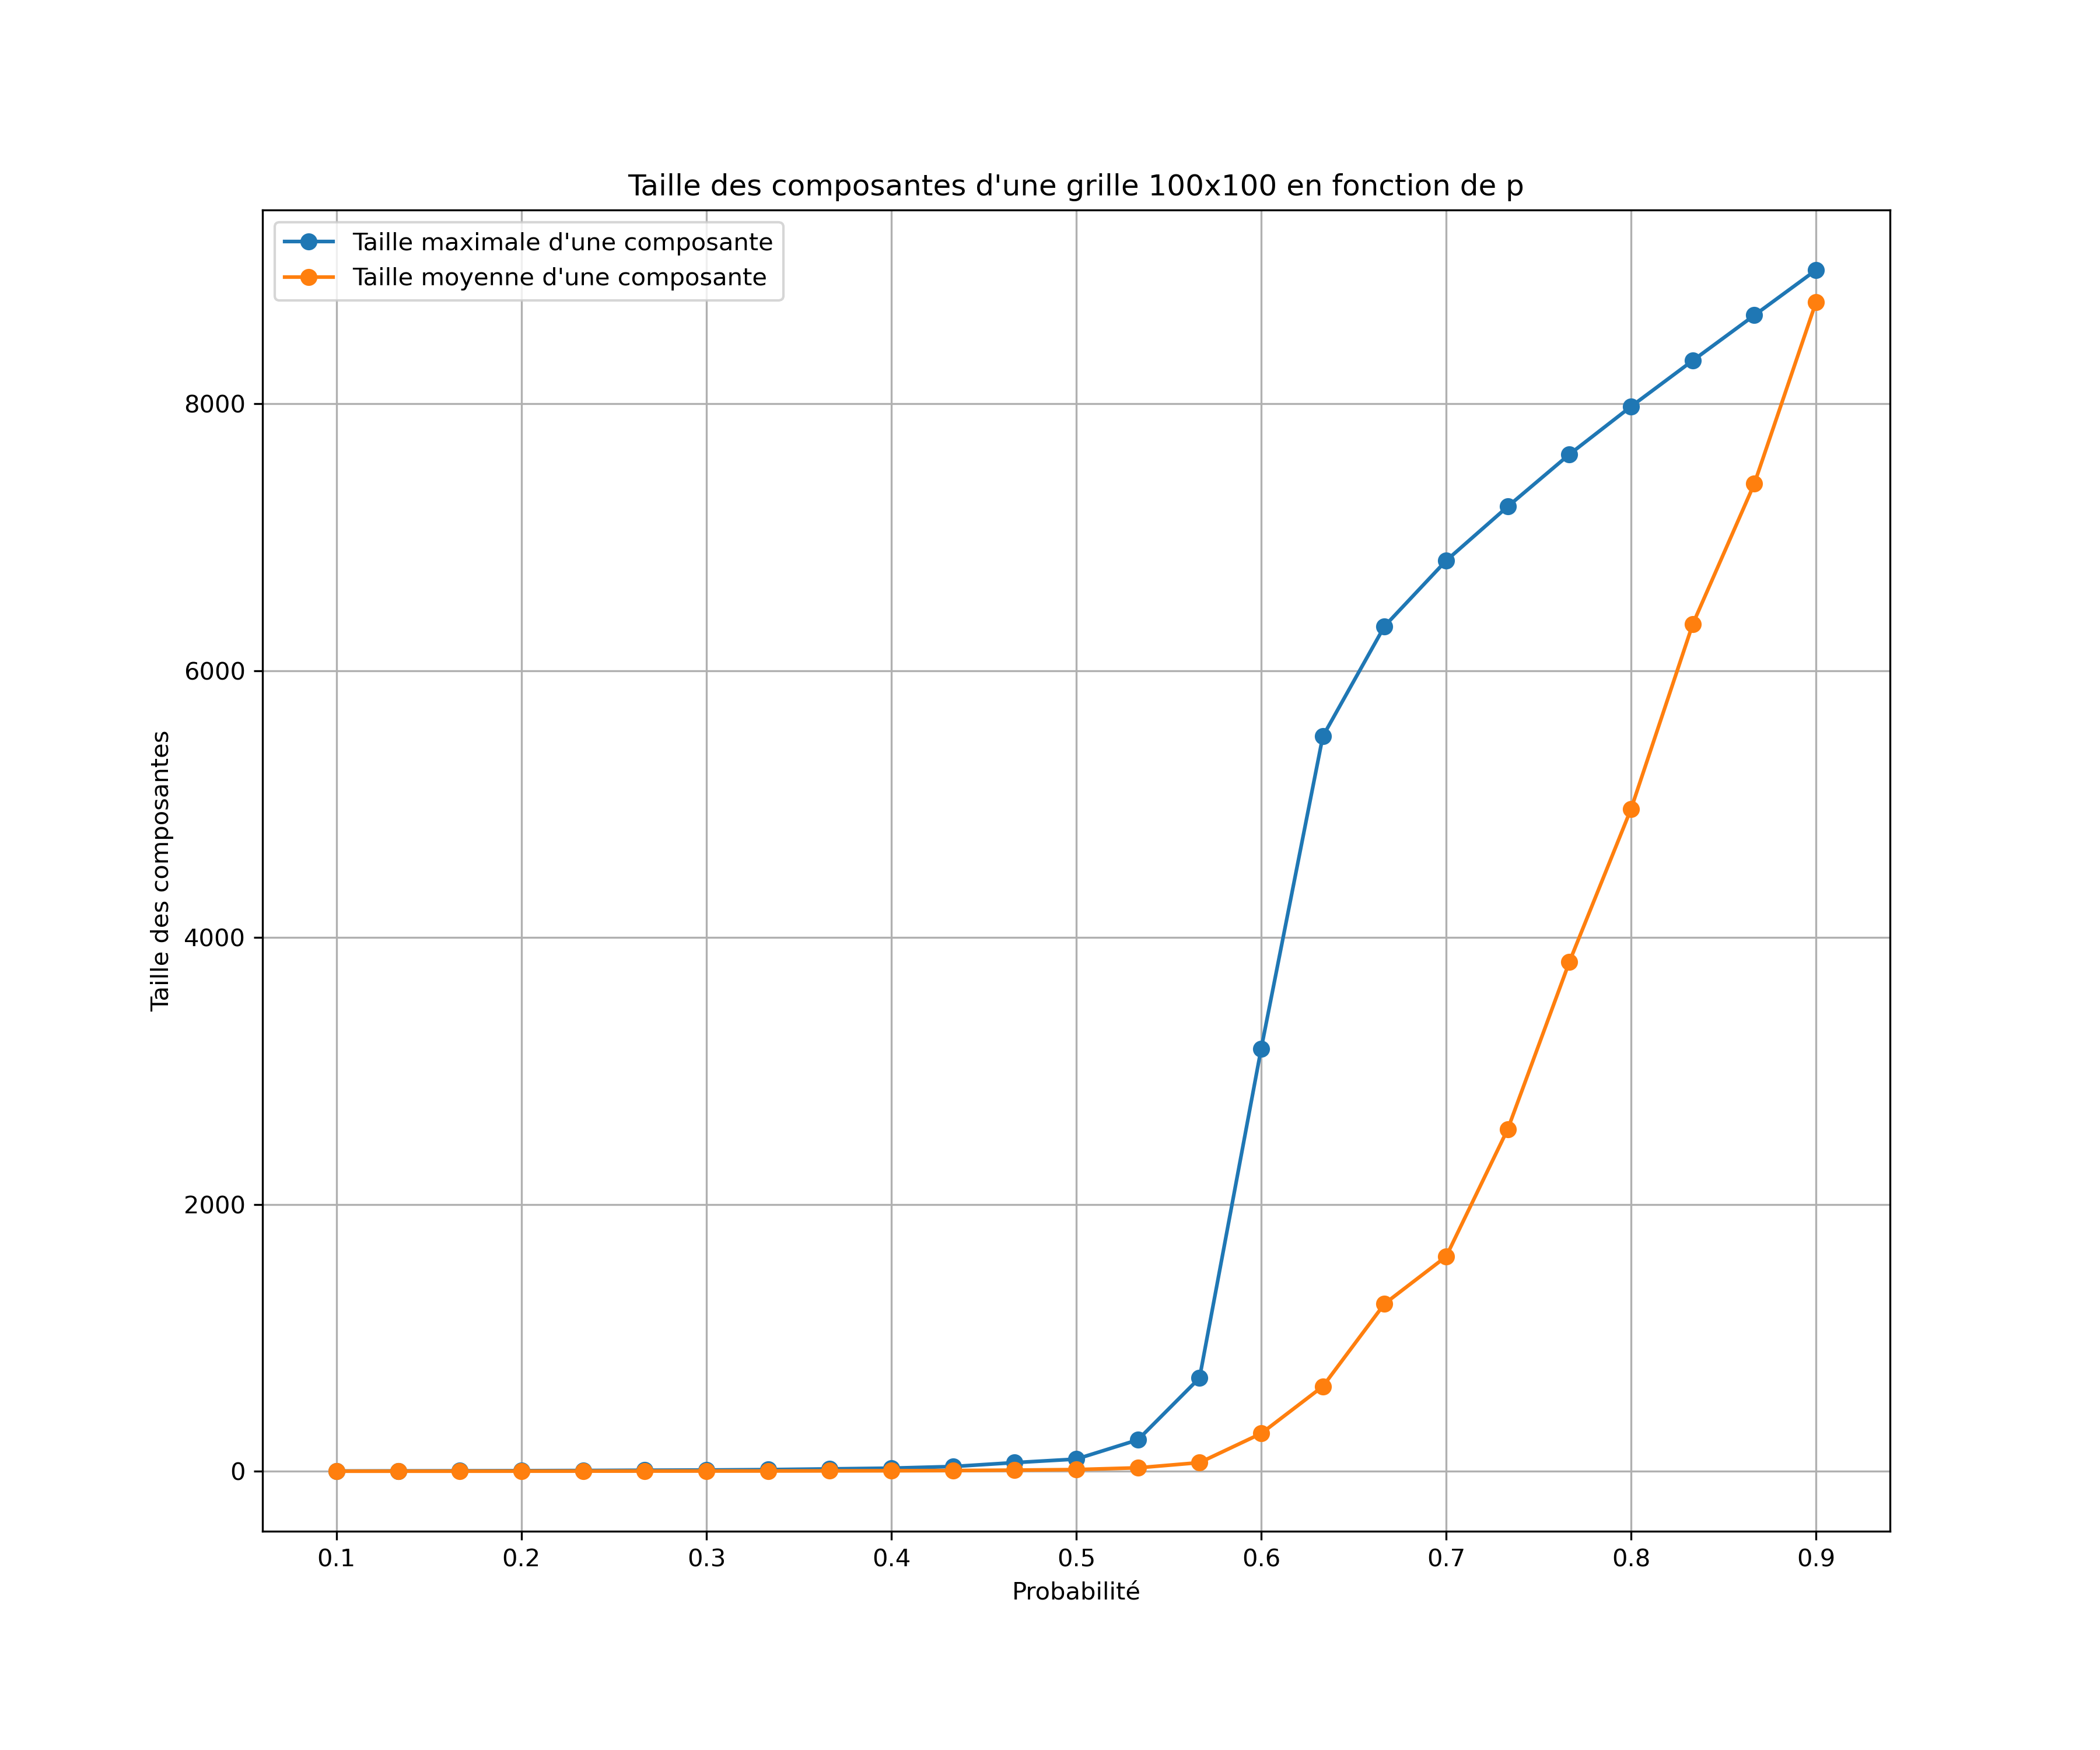
\includegraphics[width=.5\textwidth]{./Pictures/taille.png}

\caption{Profondeur, taille moyenne et maximale des composantes connexes d'une grille $100\times 100$}
\label{fig:depth_size}

\end{figure}


\subsection{Percolation dépendante}

Pour conclure cette partie, on se propose d'étudier empiriquement un second modèle de percolation, où les cases de la grille ne sont plus indépendantes entre elles. La grille sera cette fois générée de la manière suivante : on tire la première ligne où chaque case a une probabilité $p$ d'être ouverte, indépendamment des autres cases. Puis, pour les autres cases, il y a une probabilité $p'$ de conserver l'état de la cellule du dessus, et $1-p'$ d'être dans l'état opposé. Le but de cette modélisation est d'introduire de la dépendance entre les variables, et d'observer ainsi l'évolution des propriétés intrinsèques de la percolation par rapport à la modélisation précédente. \\
On observe alors un phénomène de ``fissures'' comme le montre la Figure 6. Contrairement au cas précédent, cette fois on constate de plus qu'il n'y a plus unicité de la composante connexe maximale. \\
Ensuite on estime le diagramme de phase en Figure 7, en choisissant $p=p'$ dans les simulations afin de simplifier les résultats. On remarque que la transition se fait encore plus rapidement que dans le cas classique.

\begin{figure}[htp]
    \centering
    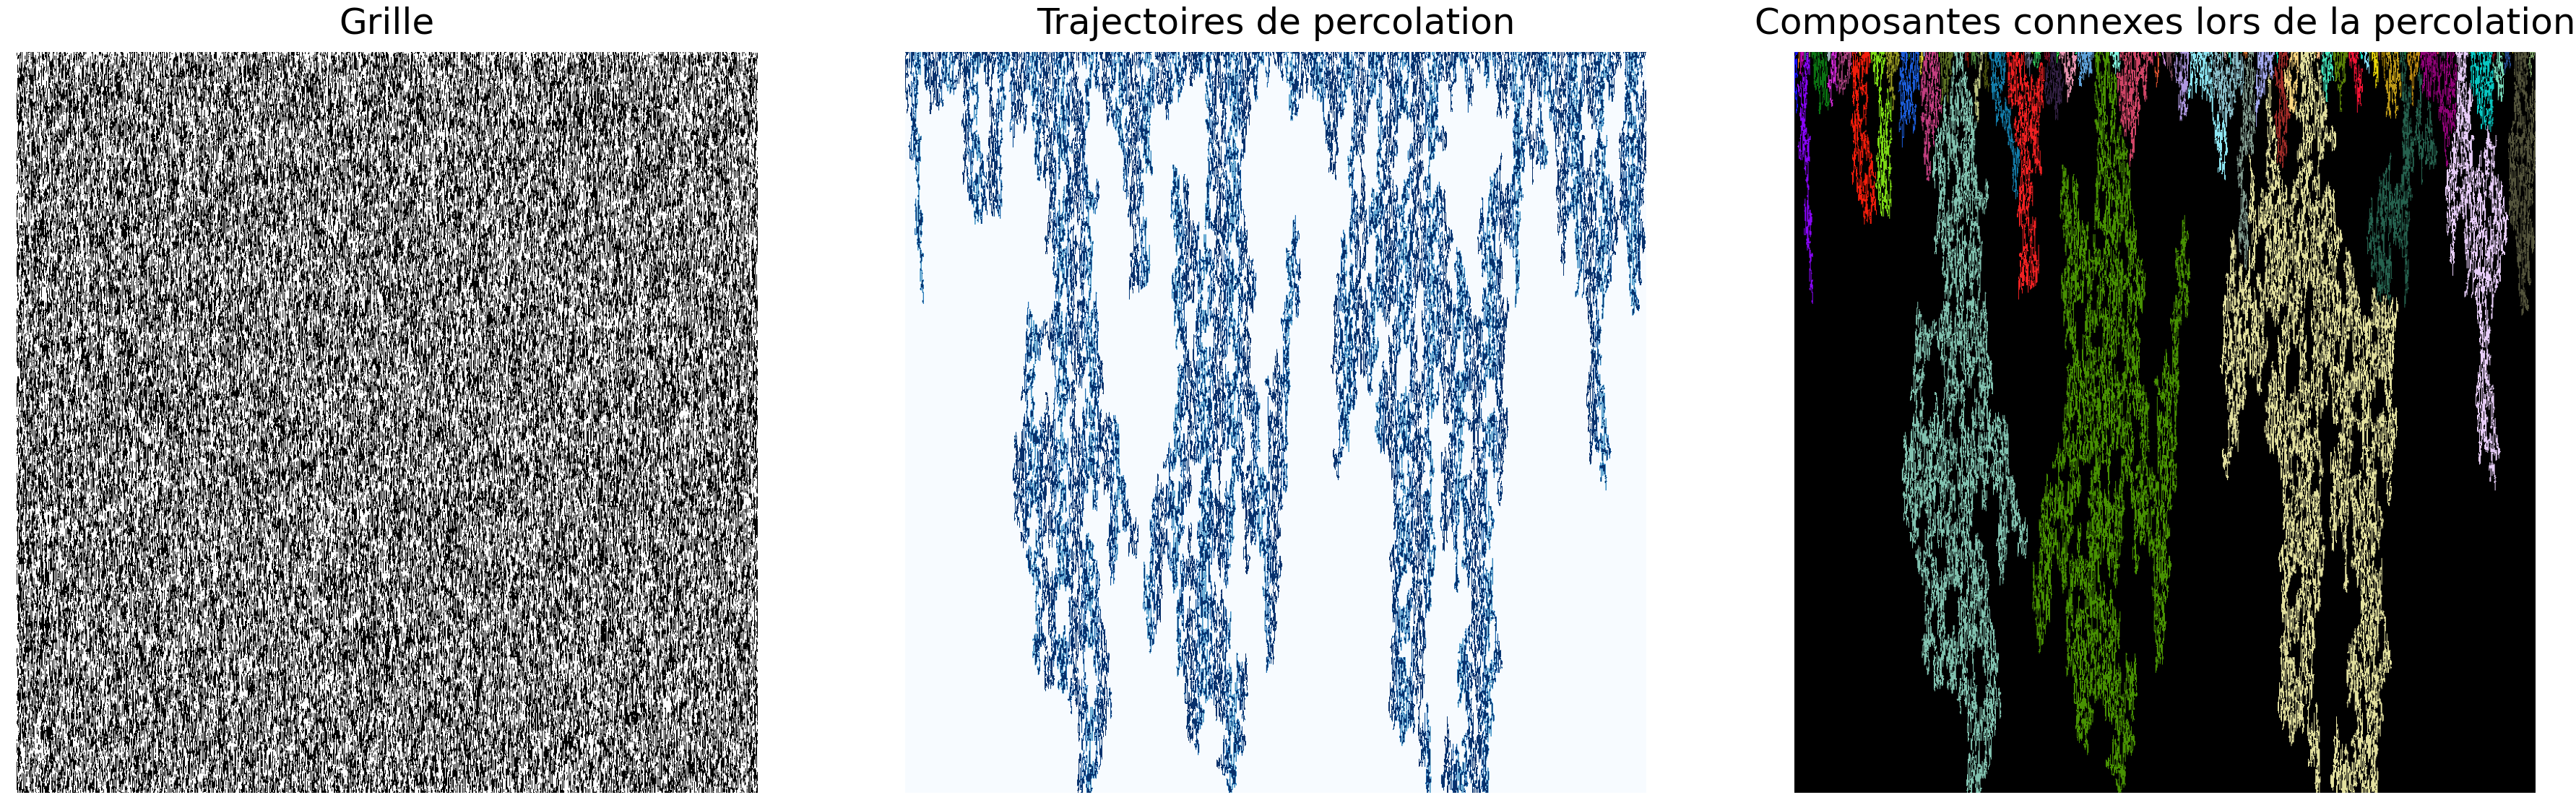
\includegraphics[width=1 \textwidth]{./Pictures/fissure.png}
    \caption{Percolation dépendante sur une grille $1000\times 1000$, avec $p=0.65$ et $p'=0.9$}
    \label{fig:fissure}
\end{figure}


\begin{figure}[H]
    \centering
    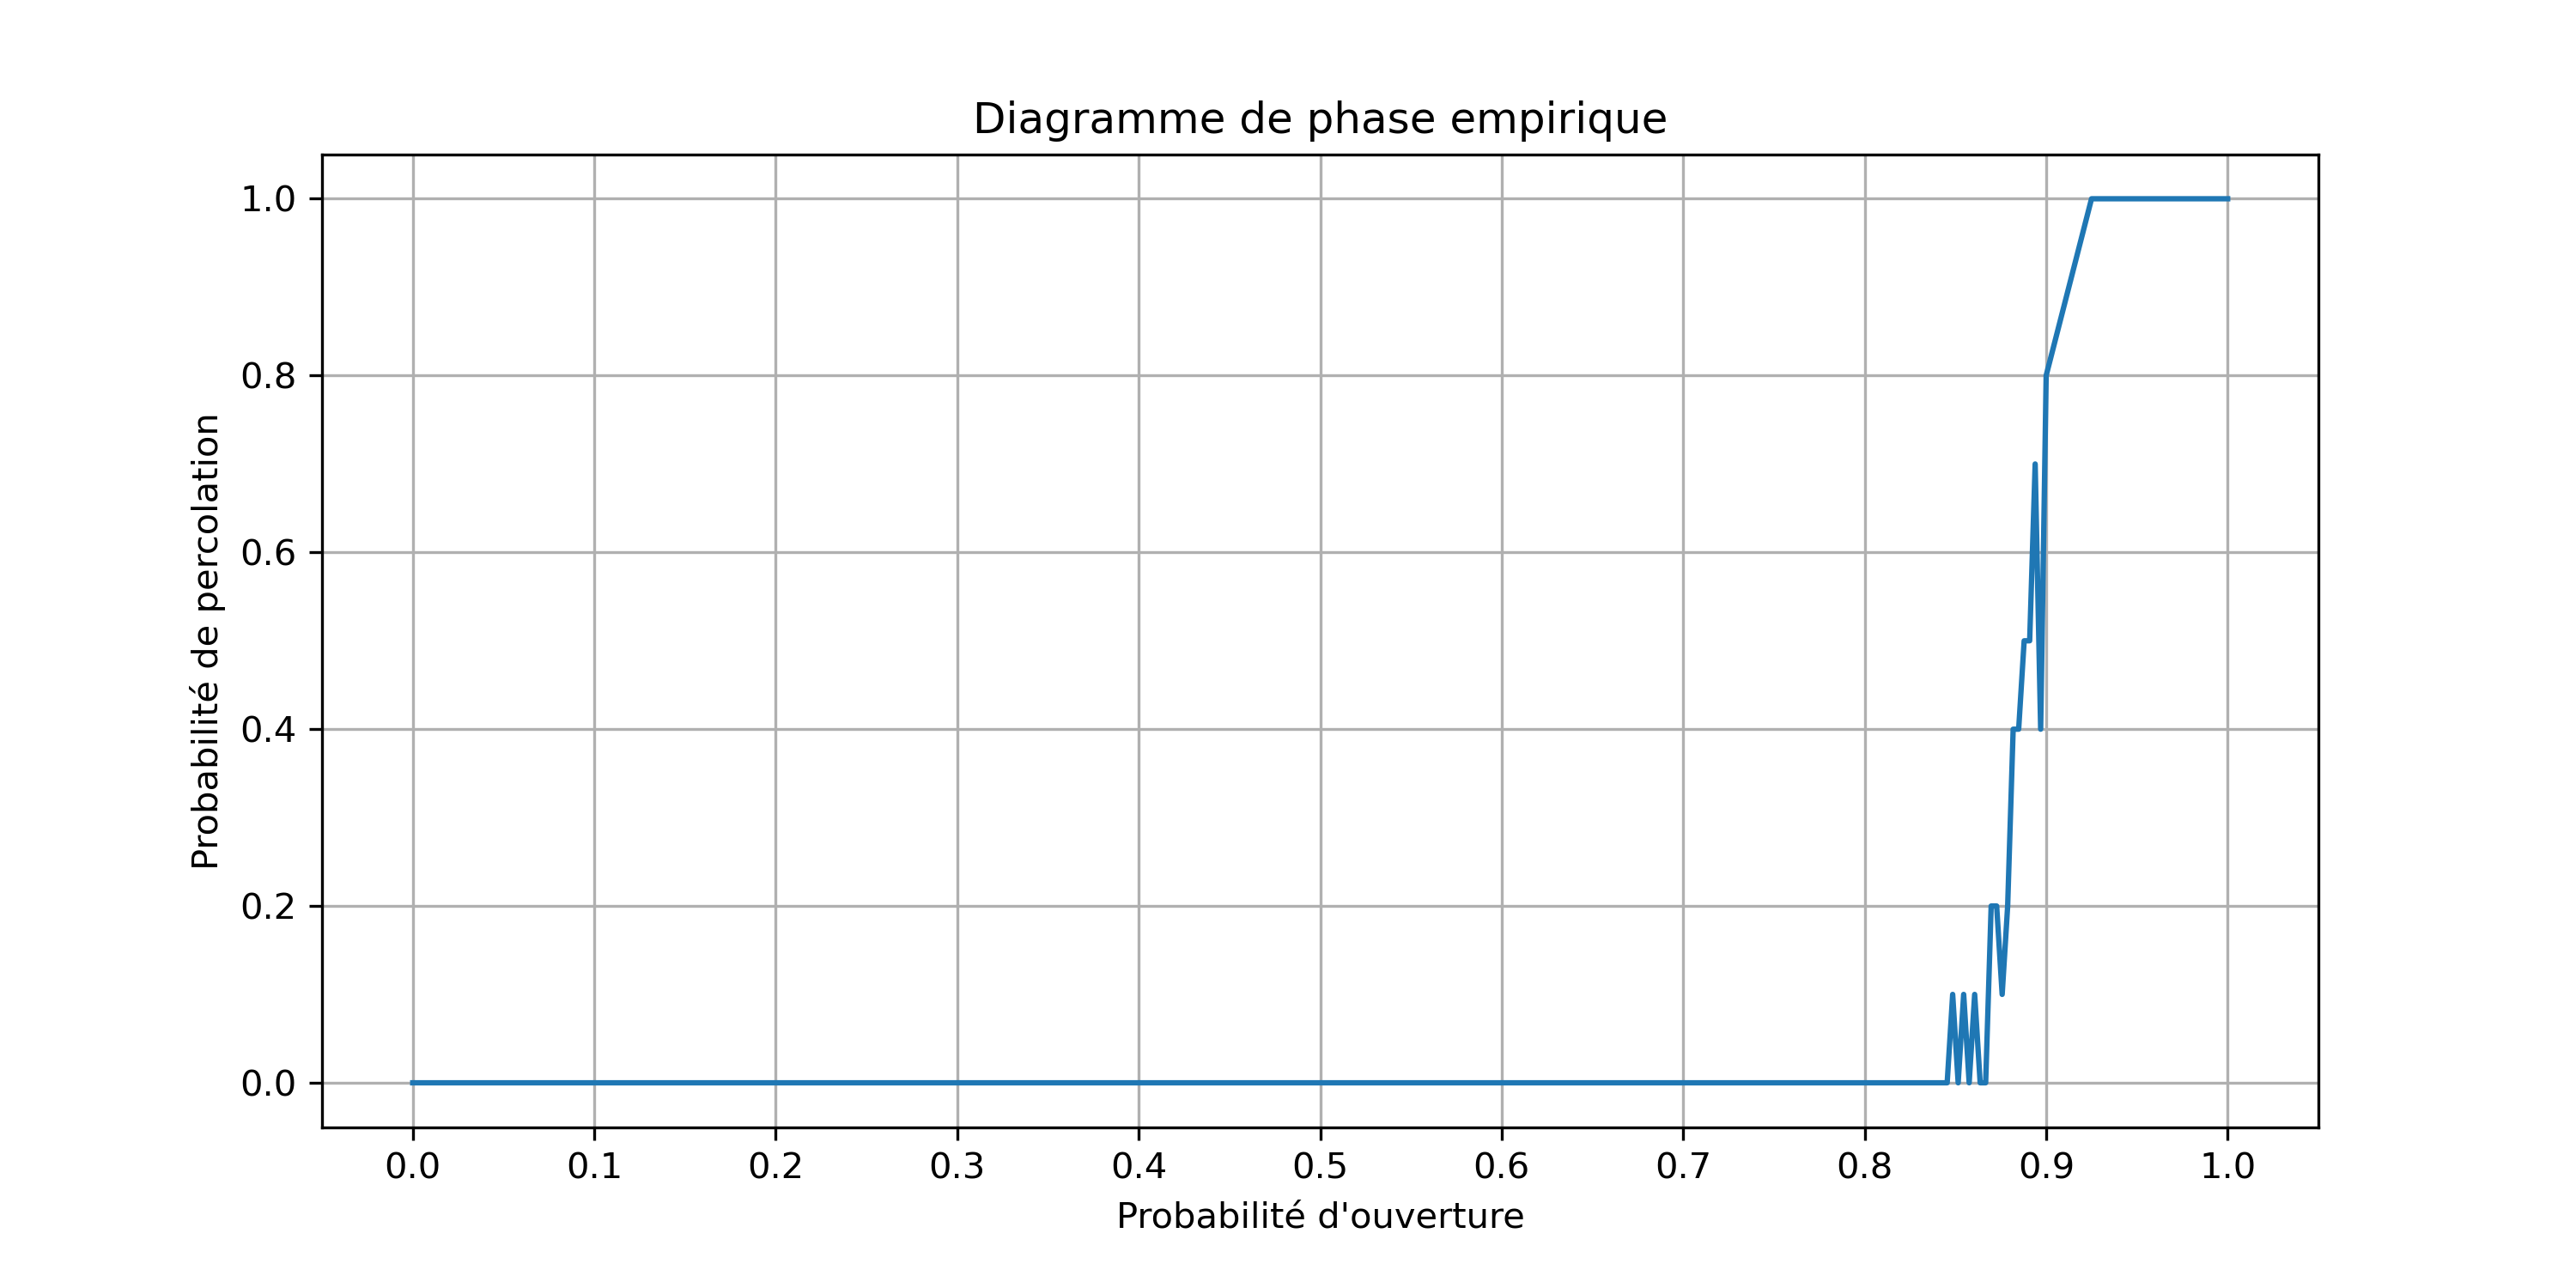
\includegraphics[width=0.6 \textwidth]{./Pictures/phase_dep.png}
    \caption{Diagramme de phase expérimental dans le cas de la percolation dépendante, régime $p=p'$}
    \label{fig:phase_dep}
\end{figure}

 De plus, on observe dans le graphique suivant que la taille moyenne et la taille maximale des composantes connexes sont globalement différentes pour des valeurs suffisamment grandes de $p$, ce qui est cohérent avec la Figure $6$, où l'on remarque que malgré l'existence de composantes connexes maximales, il reste quand même un grand nombre de petites composantes, ces dernière ne se superposant pas à cause de la modélisation choisie qui tend à préserver les cassures ou frontières entre composantes :

\begin{figure}[H]
    \centering
    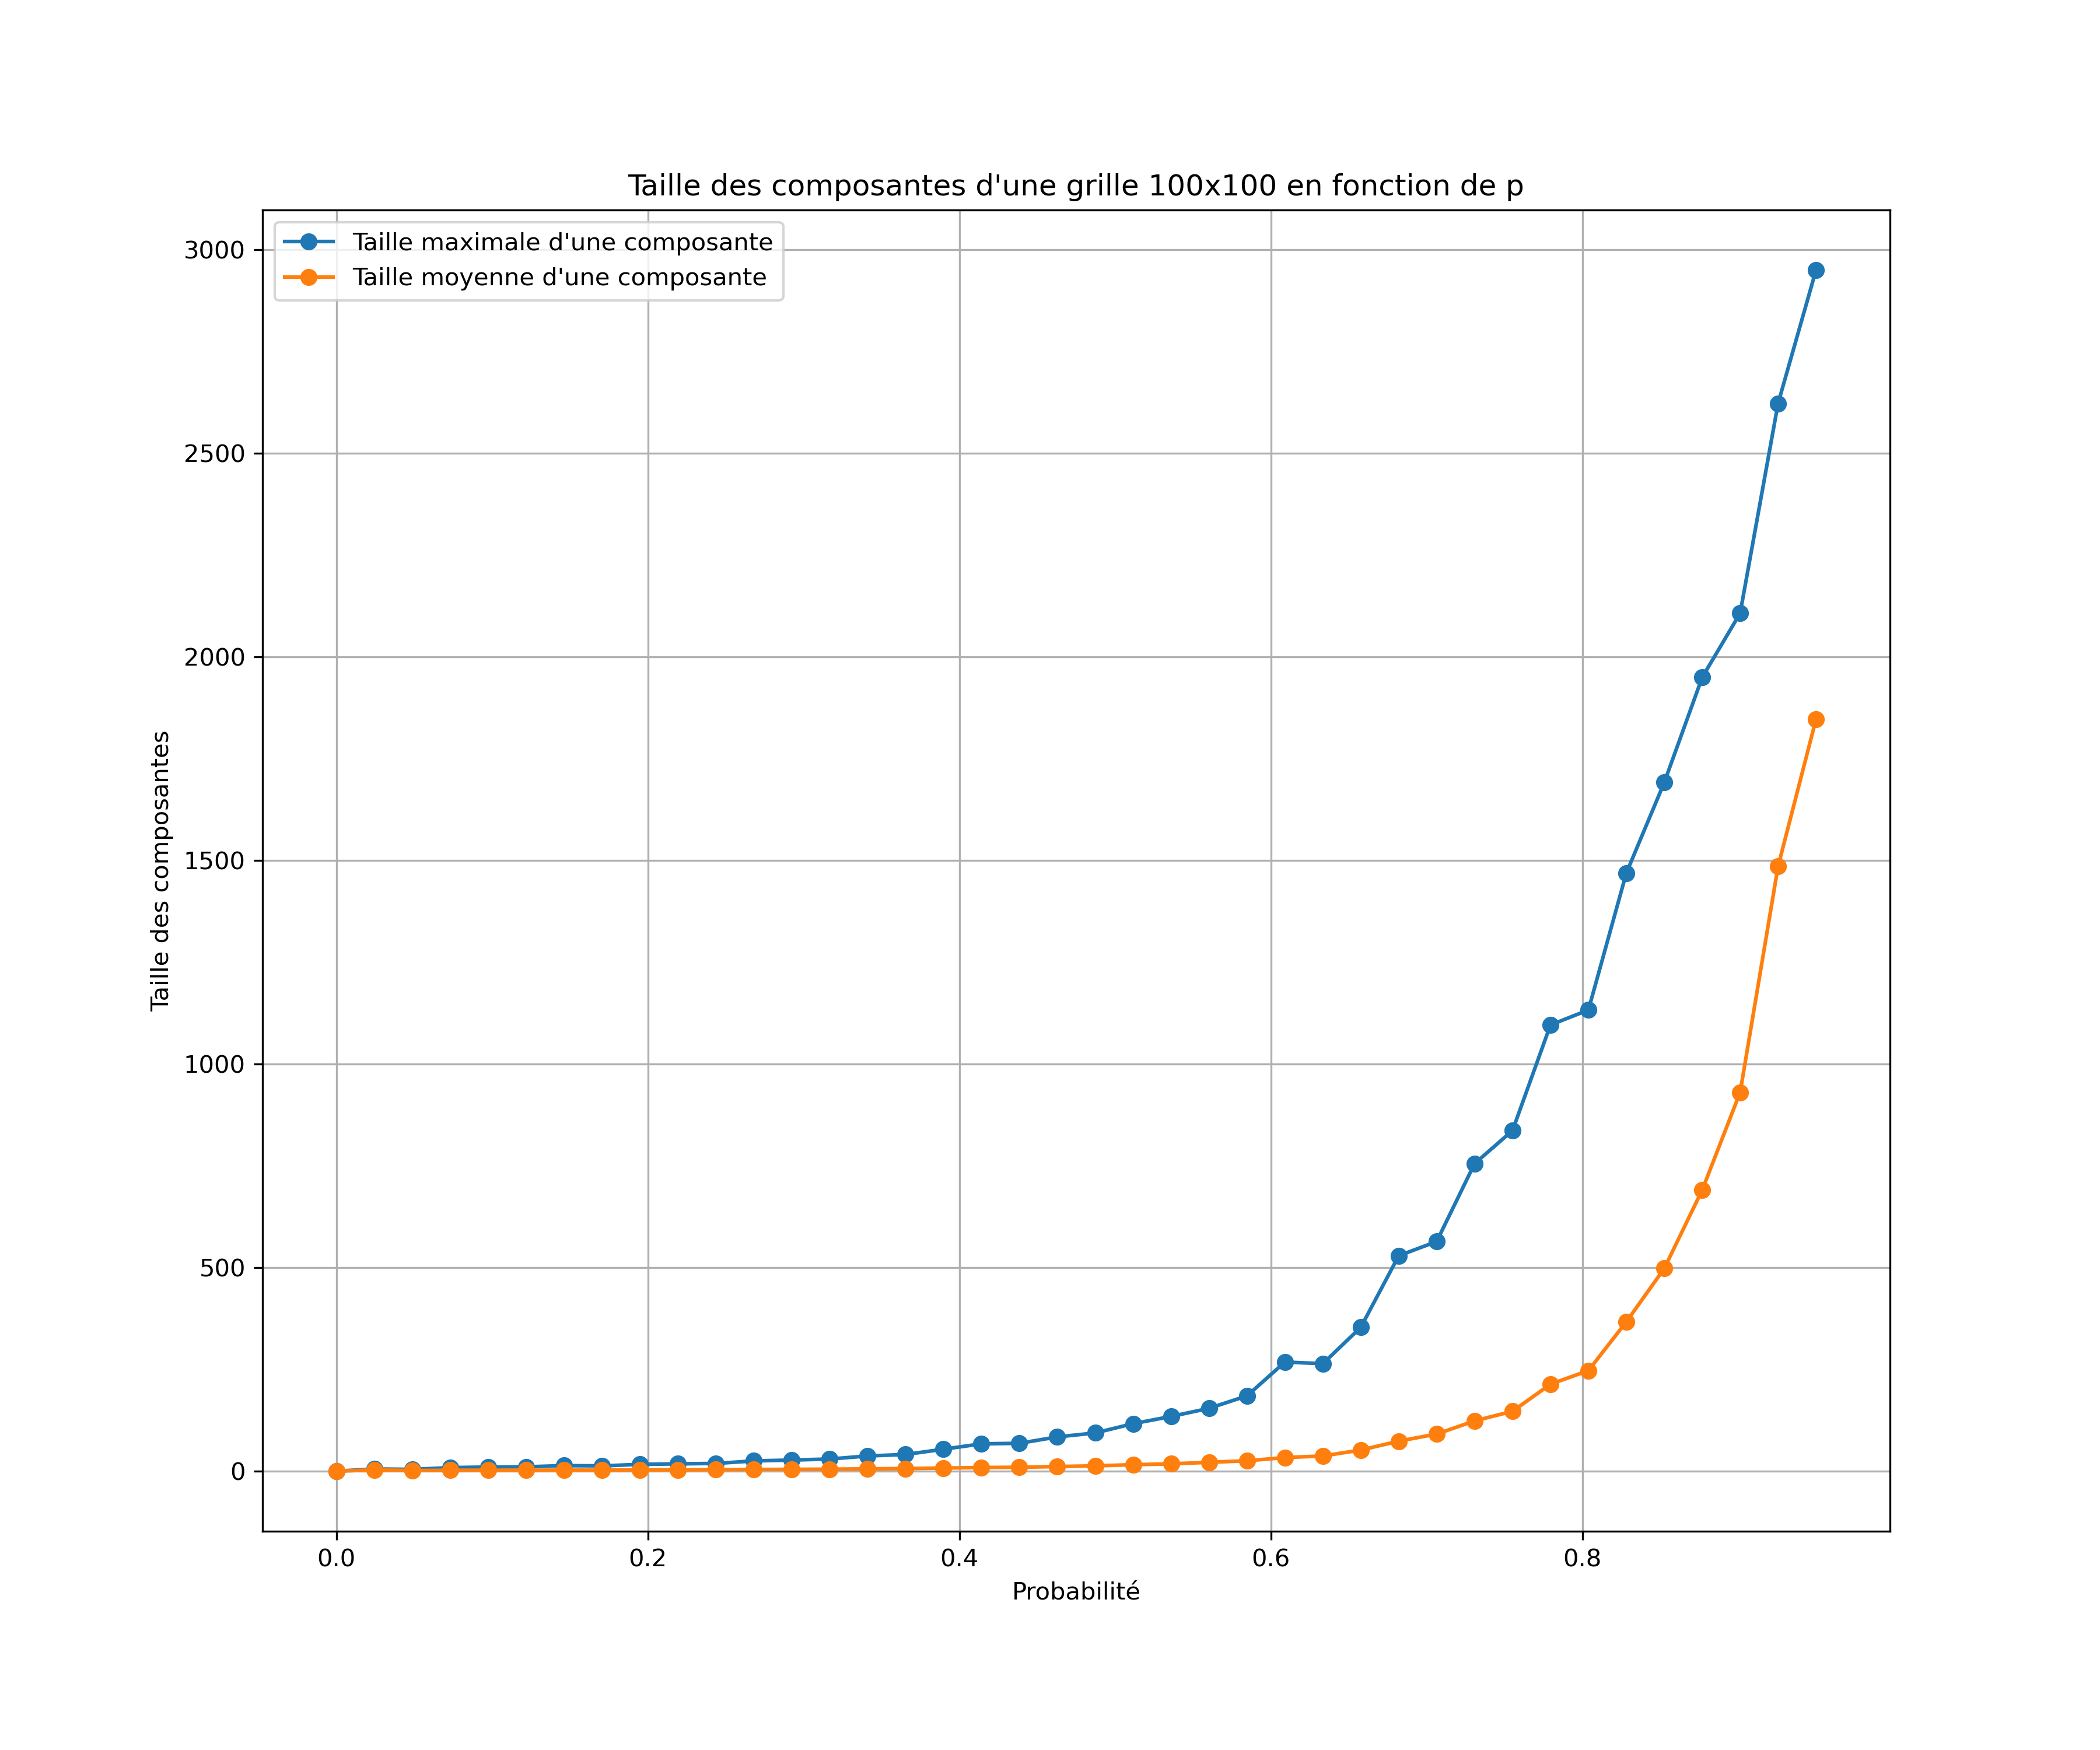
\includegraphics[width=0.5 \textwidth]{./Pictures/taille_dep.png}
    \caption{Taille moyenne et maximale des composantes connexes d'une grille $100\times 100$ générée en percolation dépendante, avec $p=p'$}
    \label{fig:phase_dep}
\end{figure}

\section{Étude théorique}

Dans cette section, nous examinerons les preuves théoriques du modèle de percolation. Tout d'abord, nous étudierons l'aspect global du diagramme de phase en nous concentrant sur $\mathbb{Z}^d$. Ensuite, nous nous pencherons sur la démonstration du théorème de Kesten, qui détermine la valeur de la probabilité critique dans $\mathbb{Z}^2$.

\subsection{Premières propositions}
\paragraph{Proposition 1 :}

On note $\Theta \left(p\right) = \mathbb{P}_p \left(\{ \exists\, 0 \leftrightarrow +\infty \}\right)$, la probabilité que $0$ soit relié à l'infini. $\Theta$ est croissante.
\\

\emph{Preuve :}

Notons $X_n$ l'ensemble des chemins de taille $n$ passant par $0$ :

\[\forall x \in X_n, \mathbb{P}_p\left(x\right) = p^n.\]

On note de même $N_n = \{$``il existe un chemin de taille $n$ passant par $0$"$ \}$ :

\[\mathbb{P}_{p'}\left(N_n\right) \ge \mathbb{P}_{p}\left(N_n\right)\Leftrightarrow p'\ge p.\]

Puisque $\Theta\left(p\right) = \underset{n \to +\infty}{\lim} \mathbb{P}_{p}\left(N_n\right)$, en passant à la limite, on trouve que $\Theta$ est croissante.

\paragraph{Proposition 2 :}
Soit $p_c$ la probabilité critique, donnée par $p_c = \sup\{p \,|\, \Theta\left(p\right) = 0\}$. On a alors $p_c\left(\mathbb{Z}^{d}\right) \ge p_c\left(\mathbb{Z}^{d+1}\right)$
\\

\emph{Preuve :}

En effet, des composantes connexes  infinies  de $\mathbb{Z}^d$ sont aussi des composantes connexes  infinies sur $\mathbb{Z}^{d+1}$.

\subsection{Prérequis au théorème de Kesten}

\paragraph{Lemme 1 :}

On note $\psi$ la fonction qui à $p$ associe la probabilité qu'il existe une composante connexe  infinie (on parlera également de nuage infini). On a $\psi\left(p\right) \in \{0,1\}$.
\\

\emph{Preuve : }

Ce résultat se montre par application de la loi du 0-1. 

On note $\left(\Gamma\left(n\right)\right)_{n\in\mathbb{N}}$ les couronnes successives de $\mathbb{Z}^2$ et $\mathcal{T}_n$ la tribu correspondant à l'ensemble des configurations dans la n-ième couronne.

L'évenement \emph{``il existe un nuage infini"} se traduit par \emph{``il existe un nuage qui traverse une infinité de couronnes"}. Donc, 

\[\forall n_0 \in \mathbb{N}, \{ \exists\, x_1 \leftrightarrow +\infty \} \in \sigma \left(\bigcup_{n\ge n_0} \mathcal{T}_n\right)\]

Finalement, $\{ \exists\, x_1 \leftrightarrow +\infty \} \in \bigcap_{n_0 \in \mathbb{N}}\sigma \left(\bigcup_{n\ge n_0} \mathcal{T}_n\right)$ qui est la tribu asymptotique de tribus indépendantes donc la loi du 0-1 s'applique.

\paragraph{Lemme 2 :} Le nuage infini (la composante connexe infinie) est presque surement unique, s'il existe. \\

\emph{Preuve :} Admis, cf partie expérimentale.

\paragraph{Lemme (Inégalité de FKG) :}

On définit la relation d'ordre partiel sur l'ensemble des configurations :

\[w_1 \le w_2 \Leftrightarrow w_2 \text{ a au moins les mêmes arêtes ouvertes que }w_1.\]

On dit que $A$ est un évenement croissant (resp. décroissant) si 

\[w_1 \le w_2 \Rightarrow \mathds{1}_A \left(w_1\right) \le \mathds{1}_A \left(w_2\right)  (\text{resp.}\ge) \]

Alors $\forall A, B$ deux évenements de même monotonie, 

\[\mathbb{P}\left(A\cap B\right) \ge \mathbb{P}\left(A\right)\mathbb{P}\left(B\right).\]


\paragraph{Graphe dual :}

On définit le graphe dual d'un graphe de $\mathbb{Z}^2$ comme un sous graphe de $\left(\mathbb{Z} + 1/2\right)\times\left(\mathbb{Z} + 1/2\right)$ avec un arête ouverte si elle ne traverse pas une arête ouverte du graphe d'origine. L'utilité de ce graphe réside dans le fait qu'en dimension 2, un chemin du graphe dual ne peut intersecter un chemin du graphe d'origine.

\paragraph{Lemme 3 : }

En régime sous-critique (ie $p<p_c$) et en notant $C$ la composante connexe de $0$, 

\[\mathbb{P}\left(|C|\ge n\right) \le \exp\left(-\alpha n\right)\]

avec $\alpha$ une constante.

\subsection{Théorème de Kesten}

On va montrer que pour $n=2$, $p_c = 1/2$ avec $\Theta\left(1/2\right) = 0$ (il n'y a pas percolation en la probabilité critique).

\paragraph{1ère étape :} 

$\Theta\left(1/2\right) = 0$

Supposons par l'absurde que $\Theta\left(1/2\right) > 0$. $\Theta\left(1/2\right) \le \psi\left(1/2\right)$ donc par le Lemme 1, $\psi\left(1/2\right) = 1$ et il existe presque sûrement un nuage infini.

On note $T(n) = [-n,n]^2$ et $\partial T(n)$ sa frontière. Par l'existence d'un nuage infini, $\exists n_0 \in \mathbb{N}$ tel que $\mathbb{P}_{1/2}\left(\partial T(n_0) \leftrightarrow +\infty\right) \ge 1 - \left(\frac{1}{8}\right)^4$ (1). En effet, $\underset{n \to +\infty}{\lim}\mathbb{P}_{1/2}\left(\partial T(n) \leftrightarrow +\infty\right) = 1$ car pour chaque configuration, on peut choisir $n$ tel que $T(n)$ intersecte le nuage infini.

Si $\{\partial T(n) \leftrightarrow +\infty\}$, alors un des quatre côtés $A_h, A_b, A_g$ et $A_d$ est relié à l'infini. Donc, 

\begin{align*}
    \mathbb{P}_{1/2}\left(\partial T(n) \cancel{\leftrightarrow} +\infty\right) &= \mathbb{P}_{1/2}\left(\overline{A_h}\cap\overline{A_b}\cap\overline{A_g}\cap\overline{A_d}\right)\\
    &\ge \prod_i \mathbb{P}_{1/2}\left(\overline{A_i}\right)  \text{ avec l'inégalité FKG}\\
    &\ge \mathbb{P}_{1/2}\left(\overline{A_h}\right)^4  \text{ par symétrie}
\end{align*}

Avec (1), on obtient $\mathbb{P}_{1/2}\left(A_i\right) \ge \frac{7}{8}$.
\\

Si on se place dans le dual de notre graphe, la démarche est identique puisque les arêtes sont ouvertes avec la même probabilité dans le dual ou dans le graphe donc $\mathbb{P}_{1/2}\left(B_i\right) \ge \frac{7}{8}$ où $B_i$ est le même évènement que  $A_i$ mais pour le dual.
\\

Intéressons nous à l'évenement $A = \{A_g \cap A_d \cap B_h \cap B_d\}$. Les inégalités précédentes montrent que $\mathbb{P}_{1/2}\left(A\right) \ge \frac{1}{2}$.
\\

Si $\{A_g \leftrightarrow +\infty\}$ et $\{A_d \leftrightarrow +\infty\}$ et par unicité du nuage infini, $A_g$ est relié à $A_d$. Il en est de même pour $B_h$ et $B_b$. Or, il est impossible qu'un chemin dans le dual intersecte un chemin dans le graphe donc $A$ est impossible, ie $\mathbb{P}_{1/2}\left(A\right)=0$, ce qui est absurde.
\\

Donc, $\Theta\left(1/2\right) = 0$ et $p_c \ge 1/2$.

\paragraph{2ème étape :}

$p_c = 1/2$

Supposons par l'absurde que $pc > 1/2$. En $p = 1/2$, on est en régime sous-critique. Reprenons la boîte $T(n)$, il y a deux scénarios :

\begin{itemize}
    \item Soit il existe un chemin reliant le haut et le bas, évenement noté $A_n$ ;
    \item ou bien il existe un chemin reliant la gauche et la droite dans le dual, évenement noté $B_n$.
\end{itemize}

On a alors, $\mathbb{P}\left(A_n \cup B_n\right) = \mathbb{P}\left(A_n\right)+\mathbb{P}\left(B_n\right)$. Or, la probabilité qu'un arête soit ouverte dans le graphe ou dans le dual est la même donc $\mathbb{P}\left(A_n\right) = \mathbb{P}\left(B_n\right)$ et finalement, $\mathbb{P}\left(A\right) = 1/2$. 
\\

Or, 
\begin{align*}
    \mathbb{P}\left(A_n\right) &= \mathbb{P}\left(\bigcup_{k=0}^n \{ (k,0) \leftrightarrow \{n\}\times[0,n]\} \right)\\
    &\le \sum_{k=0}^n \mathbb{P}\left(\{ (k,0) \leftrightarrow \{n\}\times[0,n]\}\right) \\
    &\le \left(n+1\right) \mathbb{P}\left(\{ (0,0) \leftrightarrow \{n\}\times[0,n]\}\right) \text{par symétrie du graphe} \\
    &\le \left(n+1\right) \mathbb{P}\left(\{\text{il existe un nuage de taille supérieure à $n$ autour de $0$"}\}\right)\\
    &\le \left(n+1\right)\mathbb{P}\left(\{|C|\ge n\}\right)
\end{align*}

Par le Lemme 3, il vient $\mathbb{P}\left(A\right) = 0$ ce qui est absurde.
\\

On a donc bien $p_c = 1/2$, en dimension 2.
\\

Avec la deuxième proposition 2, on montre alors qu'en dimension supérieure ou égale à $3$, $p_c \le 1/2$.

On obtient le diagrame de phase suivant déjà évoqué :


\begin{figure}[H]
    \centering
    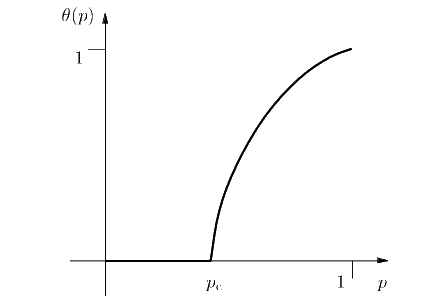
\includegraphics[width=0.4 \textwidth]{./Pictures/ph_th.png}
    \caption{Diagramme de phase théorique dans le cas de percolation standard \cite{grimmett}}
    \label{fig:phase_th}
\end{figure}


\subsection{Conclusion}

Notre étude numérique des deux modèles de percolation sur $\mathbb{Z}^2$ (dépendant et indépendant) nous a permis de mettre en lumière l'existence de phases dans le comportement de ces modèles. En effet, à partir d'une probabilité critique d'ouverture des arêtes, nous avons observé l'apparition de composantes connexes infinies. Cette analyse numérique a ainsi jeté les bases d'un diagramme de phase préliminaire.

Cette forme générale ainsi que la valeur de la probabilité critique ont ensuite été établies dans la section 3 : étude théorique. Cette dernière se concentre principalement sur la démonstration du théorème de Kesten, qui fixe la valeur de la probabilité critique pour $\mathbb{Z}^2$, en s'appuyant notamment sur une propriété vérifiée numériquement dans la première partie.


%\newpage
\printbibliography[heading=bibintoc, title={Références}]

\end{document}
